\documentclass[a4paper,12pt]{article}
\usepackage[top=1in, bottom=1in, left=1in, right=1in]{geometry}
\usepackage[normalem]{ulem}
\usepackage{graphicx}
\usepackage{setspace}
\usepackage{titlesec}
\usepackage{fontspec}
\usepackage{hyperref}
\usepackage{titlesec}
\usepackage{array}


% Set font to Times New Roman
\setmainfont{Times New Roman}

% Set line spacing
\onehalfspacing

% Set paragraph indentation
\setlength{\parindent}{6ex}

% Set headings style
\titleformat*{\section}{\large\bfseries}
\titleformat*{\subsection}{\normalsize\bfseries}

\begin{document}

\begin{titlepage}
	\centering
				        
	{\LARGE\fontsize{16}{18}\selectfont A Minor Project Final Report on 
								    
		\fontsize{16}{18}{\textbf{I-NEPAL}} \par}
				    
	\vspace{1cm}
	{\Large\fontsize{14}{16}\selectfont Submitted in Partial Fulfillment of the Requirements\\
		for the Degree of \textbf{Software Engineering}\\
		under Pokhara University\par}
				    
	% \vspace{2cm}
	\vfill
	\fontsize{14}{16}{\textbf{Submitted By:}}\\
	\fontsize{14}{16}{    Aananda Bhusal, 191701 \\
		Deepak Rana Magar, 191708 \\
		Sachit Khadka, 191722 \\
		Sibendra Timalsina, 191727 \\}
								
								
								    
		\vfill
		\fontsize{14}{16}{\textbf{Under the supervision of:}}\\
		Mr. Prakash Poudel
								    
		\vfill
		\fontsize{14}{16}{\textbf{Date:}
												    
		7th October 2023}
								    
		\vfill
								    
								    
		\begin{tabular}{@{}lcr@{}}
			
\includegraphics[width=2.7cm]{NCIT_LOGO} & \begin{tabular}[b]{@{}c@{}} 
			\multicolumn{1}{l}{\fontsize{14}{16}\selectfont \textbf{\selectfont Department of Software Engineering}} \\[0.2cm]
			\multicolumn{1}{l}{\fontsize{20}{24}\selectfont \textbf{\fontspec{Arial}\selectfont NEPAL COLLEGE OF}} \\[0.2cm]
			\multicolumn{1}{l}{\fontsize{20}{24}\selectfont \textbf{\fontspec{Arial}\selectfont \uline{INFORMATION TECHNOLOGY}}} \\
			\multicolumn{1}{l}{\fontsize{14}{16}\selectfont \fontspec{Times New Roman}\selectfont Balkumari, Lalitpur, Nepal} \\
		\end{tabular}
		\end{tabular}
								
								
								
								
		\vfill
								    
								    
		\end{titlepage}
								
		% Set font to Times New Roman
		\setmainfont{Times New Roman}
		% line spacing
		\setstretch{1.5}
		% Set paragraph indentation
		\setlength{\parindent}{0pt}
		\setlength{\parskip}{6pt}
		% binding offset set for new pages gutter margin-left
		\newgeometry{left=1in, right=1in, top=1in, bottom=1in, bindingoffset=0.5in}
								
		\pagenumbering{Roman}

        % PAGE I ACKNOWLEDGEMENT

        \newpage
		\begin{flushleft}
			\fontsize{14}{16}\selectfont\textbf{ACKNOWLEDGEMENT}
			\phantomsection
			\label{pageI}
		\end{flushleft}

  We extend our heartfelt gratitude to the college, dedicated teachers, and the esteemed faculty members of the Software Engineering department. Their collaborative efforts paved the way for the successful realization of this project. Their unwavering support and guidance were instrumental in the success of this project.

Special thanks go to our Project Supervisor Er. Prakash Poudel for his invaluable guidance and technical expertise, which played a crucial role in the development and growth of our project. His insightful suggestions propelled our project to new heights.

We are also indebted to our teachers, parents, and colleagues for their contributions, whether known or unknown. Their support and valuable insights were a cornerstone of this project's development. Thank you all for being an integral part of this journey.

\vspace{12pt}

Aananda Bhusal, 191701

Deepak Rana Magar, 191708

Sachit Khadka, 191722

Sibendra Timalsina, 191727



  
								
		% PAGE II ABSTRACT
		\newpage
		\begin{flushleft}
			\fontsize{14}{16}\selectfont\textbf{ABSTRACT}
			\phantomsection
			\label{pageII}
		\end{flushleft}
								
								
		By offering users real-time monitoring, sentiment analysis, and extensive interaction analytics, the suggested online application seeks to revolutionize Twitter data research. To keep up with the newest trends, users can log into their Twitter accounts and monitor certain subjects, keywords, or hashtags while receiving real-time updates and visualizations. Tweets are categorized as favourable, negative, or neutral by sentiment analysis algorithms, providing information on the general consensus. Users of the app can track tweet performance, reach, impressions, retweets, and likes thanks to the app's inclusion of engagement data. It enables hashtag analysis, enabling users to assess performance and pinpoint the best-performing tweets. The online app's user-friendly design, dynamic graphics, and simple navigation benefit from NextJS and Typescript construction.
								
		\vspace{6pt}
		\noindent\textbf{Keywords}: \emph{Engagement Metrics, Machine Learning, Sentiment Analysis }
								


        	% Adjust formatting for subsections
		\titleformat{\subsection}[hang]{\normalfont}{\thesubsection}{1em}{}
								
		% Set indentation for subsections
		\titlespacing{\subsection}{1.5em}{0.5em}{0.5em}


  % Adjust formatting for subsubsections
\titleformat{\subsubsection}[hang]{\normalfont}{\thesubsubsection}{1em}{}

% Set indentation for subsubsections
\titlespacing{\subsubsection}{3.5em}{0.5em}{0.5em}










  
		% PAGE II TABLE OF CONTENTS


  
		\setstretch{0.5}
				
		\newpage
				
		\begin{flushleft}
			\fontsize{14}{16}\selectfont\textbf{TABLE OF CONTENTS}
			\phantomsection
   \label{TOC}
		\end{flushleft}

            \section*{\fontsize{12}{14}\selectfont \hyperref[pageI]{ACKNOWLEDGEMENT}\protect\dotfill I}
		\addcontentsline{toc}{section}{ACKNOWLEDGEMENT}
				
		\section*{\fontsize{12}{14}\selectfont \hyperref[pageII]{ABSTRACT}\protect\dotfill II}
		\addcontentsline{toc}{section}{ABSTRACT}

   \section*{\fontsize{12}{14}\selectfont \hyperref[TOC]{TABLE OF CONTENTS}\protect\dotfill III}
		\addcontentsline{toc}{section}{TABLE OF CONTENTS}

  \section*{\fontsize{12}{14}\selectfont \hyperref[LOF]{LIST OF FIGURES}\protect\dotfill V}
		\addcontentsline{toc}{section}{LIST OF FIGURES}

  \section*{\fontsize{12}{14}\selectfont \hyperref[list]{LIST OF TABLES}\protect\dotfill VI}
		\addcontentsline{toc}{section}{LIST OF TABLES}


  % TOC - INTRODUCTION

  	\section*{\fontsize{12}{14}\selectfont \hyperref[page1]{1. 
          INTRODUCTION }\protect\dotfill 1}
		\addcontentsline{toc}{section}{INTRODUCTION}
				
		\subsection*{\fontsize{12}{14}\selectfont \hyperref[problem] {1.1 Problem Statement} \protect\dotfill 1}
		\addcontentsline{toc}{subsection}{1.1 Problem Statement}
								
		\subsection*{\fontsize{12}{14}\selectfont \hyperref[page2]{1.2 Project Objectives}\protect\dotfill 2}
		\addcontentsline{toc}{subsection}{Project Objectives}
								
		\subsection*{\fontsize{12}{14}\selectfont \hyperref[page3]{1.3 Significance Of Study}\protect\dotfill 2}
		\addcontentsline{toc}{subsection}{Significance Of Study}
								
												
		\subsection*{\fontsize{12}{14}\selectfont \hyperref[page4]{1.4. Scope and Limitation}\protect\dotfill 3}
		\addcontentsline{toc}{subsection}{Scope and Limitation}
								
		\subsubsection*{\fontsize{12}{14}\selectfont \hyperref[scope]{1.4.1. Scope} \protect\dotfill 3}
		\addcontentsline{toc}{subsubsection}{1.4.1 Scope}
								
		\subsubsection*{\fontsize{12}{14}\selectfont \hyperref[limitation]{1.4.2. Limitation} \protect\dotfill 3}
		\addcontentsline{toc}{subsubsection}{1.4.2 Limitation}


% TOC - LITERATURE REVIEW
								
			% LITERATURE REVIEW TOC
		\section*{\fontsize{12}{14}\selectfont \hyperref[page5]{2. LITERATURE REVIEW}\protect\dotfill 4}
		\addcontentsline{toc}{section}{LITERATURE REVIEW}

  % TOC - METHODOLOGY
								
		\section*{\fontsize{12}{14}\selectfont \hyperref[page6]{3. METHODOLOGY}\protect\dotfill 7}
		\addcontentsline{toc}{section}{METHODOLOGY}
								
		\subsection*{\fontsize{12}{14}\selectfont \hyperref[SDLC]{3.1 Software Model} \protect\dotfill 7}
		\addcontentsline{toc}{subsection}{3.1 PROPOSED SOFTWARE MODEL}
								
		\subsection*{\fontsize{12}{14}\selectfont \hyperref[architecture]{3.2 System Architecture} \protect\dotfill 9}
		\addcontentsline{toc}{subsection}{3.2 SYSTEM ARCHITECTURE}

  \subsection*{\fontsize{12}{14}\selectfont \hyperref[bert]{3.3 Implemented Model} \protect\dotfill 11}
		\addcontentsline{toc}{subsection}{3.3 Implemented Model}
								
		\subsection*{\fontsize{12}{14}\selectfont \hyperref[usecase]{3.4 UseCase Diagram} \protect\dotfill 12}
		\addcontentsline{toc}{subsection}{3.3 USECASE DIAGRAM}
								
		\subsection*{\fontsize{12}{14}\selectfont \hyperref[activity]{3.5 Activity Diagram} \protect\dotfill 13}
		\addcontentsline{toc}{subsection}{3.4 Activity Diagram}
  
        \subsection*{\fontsize{12}{14}\selectfont \hyperref[sequence]{3.6 Sequence Diagram} \protect\dotfill 14}
		\addcontentsline{toc}{subsection}{3.4 Sequence Diagram}



  % TOC - REQUIREMENT ANALYSIS

				
		\section*{\fontsize{12}{14}\selectfont \hyperref[requirement]{4. REQUIREMENT ANALYSIS}\protect\dotfill 14}
		\addcontentsline{toc}{section}{4. REQUIREMENT ANALYSIS}  
				
		\subsection*{\fontsize{12}{14}\selectfont \hyperref[fun]{4.1 Functional Requirements} \protect\dotfill 14}
		\addcontentsline{toc}{subsection}{4.1 Functional Requirements}
				
		\subsection*{\fontsize{12}{14}\selectfont \hyperref[nonfun]{4.2.Non-Functional Requirements} \protect\dotfill 15}
		\addcontentsline{toc}{subsection}{4.2.Non-Functional Requirements}



     
		\subsection*{\fontsize{12}{14}\selectfont \hyperref[soft]{4.3 Software Requirements} \protect\dotfill 15}
		\addcontentsline{toc}{subsection}{4.3. Software Requirements}

        \subsubsection*{\fontsize{12}{14}\selectfont \hyperref[next]{4.3.1 NextJS} \protect\dotfill 15}
		\addcontentsline{toc}{subsubsection}{4.3.1 NextJS}
								
		\subsubsection*{\fontsize{12}{14}\selectfont \hyperref[redux]{4.3.2 Redux} \protect\dotfill 115}
		\addcontentsline{toc}{subsubsection}{4.3.2 Redux}

\newpage	
  
  \subsubsection*{\fontsize{12}{14}\selectfont \hyperref[tweetapi]{4.3.3 Twitter API} \protect\dotfill 16}
		\addcontentsline{toc}{subsubsection}{4.3.3 Twitter API}
  
	

		\subsubsection*{\fontsize{12}{14}\selectfont \hyperref[torch]{4.3.4 Torch} \protect\dotfill 16}
		\addcontentsline{toc}{subsubsection}{4.3.4 Torch}

     

  \subsubsection*{\fontsize{12}{14}\selectfont \hyperref[pandas]{4.3.5 Pandas} \protect\dotfill 16}
		\addcontentsline{toc}{subsubsection}{4.3.5 Pandas}
								
		\subsubsection*{\fontsize{12}{14}\selectfont \hyperref[transform]{4.3.6 Transformers} \protect\dotfill 16}
		\addcontentsline{toc}{subsubsection}{4.3.6 Transformers}

  \subsubsection*{\fontsize{12}{14}\selectfont \hyperref[mat]{4.3.7 MatPlotlib} \protect\dotfill 16}
		\addcontentsline{toc}{subsubsection}{4.3.7 MatPlotlib}
								
		\subsubsection*{\fontsize{12}{14}\selectfont \hyperref[latex]{4.3.8 LaTEX} \protect\dotfill 17}
		\addcontentsline{toc}{subsubsection}{4.3.8 LaTex}

  		\subsubsection*{\fontsize{12}{14}\selectfont \hyperref[mongo]{4.3.9 MongoDB} \protect\dotfill 17}
		\addcontentsline{toc}{subsubsection}{4.3.9 MongoDB}


  % TOC - IMPLEMENTATION DETAILS
  \section*{\fontsize{12}{14}\selectfont \hyperref[implementation]{5. IMPLEMENTATION DETAILS}\protect\dotfill 18}
		\addcontentsline{toc}{section}{5. IMPLEMENTATION DETAILS}

  \subsection*{\fontsize{12}{14}\selectfont \hyperref[ai]{5.1 AI Model} \protect\dotfill 18}
		\addcontentsline{toc}{subsection}{5.1 AI Model}
				
		\subsubsection*{\fontsize{12}{14}\selectfont \hyperref[data]{5.1.1 DataSet} \protect\dotfill 18}
		\addcontentsline{toc}{subsubsection}{5.1.1 DataSet}

  \subsubsection*{\fontsize{12}{14}\selectfont \hyperref[model]{5.1.2 Model} \protect\dotfill 18}
		\addcontentsline{toc}{subsubsection}{5.1.2 Model}

    \subsubsection*{\fontsize{12}{14}\selectfont \hyperref[preprocess]{5.1.3 Preprocessing} \protect\dotfill 19}
		\addcontentsline{toc}{subsubsection}{5.1.3 Preprocessing}

   \subsubsection*{\fontsize{12}{14}\selectfont \hyperref[train]{5.1.4 Training} \protect\dotfill 19}
		\addcontentsline{toc}{subsubsection}{5.1.4 Training}


\subsection*{\fontsize{12}{14}\selectfont \hyperref[train]{5.2 User Interface Development} \protect\dotfill 19}
		\addcontentsline{toc}{subsection}{5.2 User Interface Development}

  \subsection*{\fontsize{12}{14}\selectfont \hyperref[train]{5.3 Database} \protect\dotfill 20}
		\addcontentsline{toc}{subsection}{5.3 Database}

  




% TOC - RESULT AND ANALYSIS
\section*{\fontsize{12}{14}\selectfont \hyperref[page7]{6. RESULT AND ANALYSIS}\protect\dotfill 21}
		\addcontentsline{toc}{section}{4. REQUIREMENT ANALYSIS}

  \subsection*{\fontsize{12}{14}\selectfont \hyperref[train]{6.1 Training Progress and Evaluation Metrics} \protect\dotfill 21}
		\addcontentsline{toc}{subsection}{6.1 Training Progress and Evaluation Metrics}
				
		\subsubsection*{\fontsize{12}{14}\selectfont \hyperref[lvg]{6.1.1 Loss Value Graph} \protect\dotfill 21}
		\addcontentsline{toc}{subsubsection}{6.1.1 Loss Value Graph}

  \subsubsection*{\fontsize{12}{14}\selectfont \hyperref[avg]{6.1.2 Accuracy Value Graph} \protect\dotfill 22}
		\addcontentsline{toc}{subsubsection}{6.1.2 Accuracy Value Graph}

\subsection*{\fontsize{12}{14}\selectfont \hyperref[train]{6.2 Data Visualisation} \protect\dotfill 22}
		\addcontentsline{toc}{subsection}{6.2 Data Visualisation}




  % TOC - CONCLUSION
				
		\section*{\fontsize{12}{14}\selectfont \hyperref[conclusion]{7. CONCLUSION}\protect\dotfill 24}
		\addcontentsline{toc}{section}{7. CONCLUSION}
				
		
		


% TOC - FURTHER WORKS
		\section*{\fontsize{12}{14}\selectfont \hyperref[future]{8. FUTURE ENHANCEMENTS}\protect\dotfill 25}
		\addcontentsline{toc}{section}{8. FUTURE ENHANCEMENTS}
		
		 
		
		
% TOC - PROJECT TIME AND SCHEDULE
						
		\section*{\fontsize{12}{14}\selectfont \hyperref[task]{9. PROJECT TASK AND TIME SCHEDULE}\protect\dotfill 26}
		\addcontentsline{toc}{section}{PROJECT TASK AND TIME SCHEDULE}


% TOC - REFERENCES
								
		\section*{\fontsize{12}{14}\selectfont \hyperref[reference]{REFERENCES}\protect\dotfill 27}
		\addcontentsline{toc}{section}{REFERENCES}









        
								
		% PAGE II LIST OF FIGURES
		\newpage
		\begin{flushleft}
			\fontsize{14}{16}\selectfont\textbf{LIST OF FIGURES}
   \phantomsection
			\label{LOF}
		\end{flushleft}
								
		\section*{\fontsize{12}{14}\selectfont \hyperref[incremental]{1. INCREMENTAL MODEL}\protect\dotfill 7}
		\addcontentsline{toc}{section}{INCREMENTAL MODEL}
								
		\section*{\fontsize{12}{14}\selectfont \hyperref[block-diagram]{2. BLOCK DIAGRAM}\protect\dotfill 9}
		\addcontentsline{toc}{section}{BLOCK DIAGRAM}
								
		\section*{\fontsize{12}{14}\selectfont \hyperref[usecase_diagram]{3. USECASE DIAGRAM}\protect\dotfill 11}
		\addcontentsline{toc}{section}{USECASE DIAGRAM}

  
  		\section*{\fontsize{12}{14}\selectfont \hyperref[activitydiagram]{4. ACTIVITY DIAGRAM}\protect\dotfill 12}
		\addcontentsline{toc}{section}{4. ACTIVITY DIAGRAM}
								
		\section*{\fontsize{12}{14}\selectfont \hyperref[sequencediagram]{5. SEQUENCE DIAGRAM}\protect\dotfill 13}
		\addcontentsline{toc}{section}{5. SEQUENCE DIAGRAM}

            \section*{\fontsize{12}{14}\selectfont \hyperref[dataset]{6. DATASET}\protect\dotfill 18}
		\addcontentsline{toc}{section}{6. DATASET}

         \section*{\fontsize{12}{14}\selectfont \hyperref[loss]{7. LOSS VALUE GRAPH}\protect\dotfill 21}
		\addcontentsline{toc}{section}{7. LOSS VALUE GRAPH}

        \section*{\fontsize{12}{14}\selectfont \hyperref[acc]{8. ACCURACY VALUE GRAPH}\protect\dotfill 22}
		\addcontentsline{toc}{section}{{8. ACCURACY VALUE GRAPH}

   \section*{\fontsize{12}{14}\selectfont \hyperref[per]{9. TWEET PERFORMANCE GRPAH}\protect\dotfill 23}
		\addcontentsline{toc}{section}{{9. TWEET PERFORMANCE GRPAH}

   \section*{\fontsize{12}{14}\selectfont \hyperref[sen]{10. SENTIMENT ANALYSIS GRAPH}\protect\dotfill 23}
		\addcontentsline{toc}{section}{{10. SENTIMENT ANALYSIS GRAPH}

  	    \section*{\fontsize{12}{14}\selectfont \hyperref[gantt]{11. GANTT CHART}\protect\dotfill 26}
		\addcontentsline{toc}{section}{9. GANTT CHART}
				
    \newpage



%                         LIST OF TABLE

\newpage
		\begin{flushleft}
			\fontsize{14}{16}\selectfont\textbf{LIST OF TABLE}
   \phantomsection
			\label{list}
		\end{flushleft}
								
		\section*{\fontsize{12}{14}\selectfont \hyperref[tablel1]{1. FUNCTIONAL REQUIREMENTS}\protect\dotfill 14}
		\addcontentsline{toc}{section}{1. FUNCTIONAL REQUIREMENTS}



\newpage

% formatting sections after TOC


% subsubsection
    \titleformat{\subsubsection}[hang]{\normalfont\bfseries}{\thesubsubsection}{1em}{}

% subsection
\titleformat{\subsection}[hang]{\normalfont\bfseries}{\thesubsection}{1em}{}





%                MAIN CONTENT STARTS FROM HERE
    

% ARABIC PAGE NUMBERING STARTS
    \setstretch{1.5}
		\pagenumbering{arabic}




















  

%                         PAGE-1 -> INTRODUCTION
      
      \setstretch{1.5}
		\pagenumbering{arabic}
								
		\begin{flushleft}
			\fontsize{14}{16}\selectfont\textbf{1. INTRODUCTION}
			\phantomsection
			\label{page1}
		\end{flushleft}
  I-NEPAL, or Insights Nepal, is an innovative project focused on developing a web platform that harnesses the capabilities of Twitter's API. Its aim is to provide users with a comprehensive view of their Twitter account, along with clear data visualizations and advanced analysis of tweet sentiments. This platform is specifically designed to cater to the needs of the Nepali context, where there is currently a lack of specialized tools for analyzing and visualizing Twitter data. By filling this gap, I-NEPAL aims to give users a tailored and powerful solution for gaining valuable insights into their Twitter presence.

The main objective of I-NEPAL is to offer users an easy-to-use interface that taps into the extensive functionalities of Twitter's API. This grants users access to a wealth of information about their Twitter activity, including detailed visual representations of their account's performance metrics. Additionally, the platform incorporates advanced algorithms for sentiment analysis, capable of processing Nepali Devanagari text found in tweets. This unique feature allows users to gain deep insights into how their followers perceive and engage with their tweets. With I-NEPAL, users can make well-informed decisions to refine and enhance their Twitter strategies, addressing a crucial need in the Nepali social media landscape.


								
		
%                       1.1 PROBLEM STATEMENT
		
  \begin{flushleft}
			\fontsize{13}{15}\selectfont\textbf{1.1 Problem Statement }
			\phantomsection
			\label{problem}
		\end{flushleft}

								
		
								
		In Nepal, present constraints in monitoring and interpreting Twitter data limit effective research and decision-making. Existing solutions are deficient in terms of real-time monitoring, sentiment analysis, complete interaction analytics, and user-friendly design for Nepali context and Language. Users are unable to track specific issues, interpret sentiment, evaluate tweet performance, or undertake hashtag analysis as a result. A full admin panel with sentiment analysis, interaction statistics, and a user-friendly interface is required to revolutionize Twitter data research in Nepal.
								
		Enable people and organizations in Nepal to assess the performance and impact of their Twitter activity by providing comprehensive engagement data, such as reach, impressions, retweets, and likes. Enable hashtag analysis as well to find the best-performing hashtags that are pertinent to Nepal.
								
				
				    
%                         1.2 PROJECT OBJECTIVES
				
						
		\begin{flushleft}
			\fontsize{13}{15}\selectfont\textbf{1.2. Project Objectives}
			\phantomsection
			\label{page2}
		\end{flushleft}
								
		\begin{enumerate}
			\item To develop an intuitive online web application that provide  updates by monitoring and analyzing Twitter data relevant to Nepal.
			         
			\item To empower users to track their tweet performance.
			      						
		\end{enumerate}
								
								
								
%                    1.3 SIGNIFICANCE OF STUDY 
		
								
		\begin{flushleft}
			\fontsize{13}{15}\selectfont\textbf{1.3 Significance of study}
			\phantomsection
			\label{page3}
		\end{flushleft}
								
		\begin{enumerate}
												
			\item  Closing the data gap: By creating a dedicated Twitter analysis software for Nepal, the lack of real-time Twitter data accessibility is addressed, and the knowledge gap on the dynamics of the Nepalese population is filled. This can help researchers, companies, and people to make data-driven decisions and obtain a deeper understanding of Nepalese society by revealing the views, opinions, and trends of Nepalese Twitter users.
			      			      			      			      
			\item Improved decision-making and communication: The app supports wise decision-making and successful communication strategies by tracking and evaluating sentiment and public opinion on numerous subjects, events, and social concerns in Nepal. With the help of this study, anyone will be better able to grasp public mood, take appropriate action, and modify their messaging to make projects and growth strategies more effective and focused.
			      			      			      			      
			\item Social media plans are strengthened by the app's extensive engagement analytics which enable people and organizations in Nepal to assess the effectiveness and impact of their Twitter activity. This study gives consumers the resources they need to better their social media strategy, spot opportunities for development, and keep up with the competition. It makes it possible for people, companies, and organizations to interact with their customers, expand their reach, and establish a solid online presence in the Nepalese Twitter community thus making the market more competitive.
			      			      			      			      
		\end{enumerate}

  
						
%                        1.4 SCOPE AND LIMITATION 

  \newpage
								
		\begin{flushleft}
			\fontsize{13}{15}\selectfont\textbf{1.4. Scope and Limitation}
			\phantomsection
			\label{page4}
		\end{flushleft}
								
		\begin{flushleft}
			\fontsize{13}{15}\selectfont\textbf{1.4.1 Scope}
			\phantomsection
			\label{scope}
		\end{flushleft}
								
		\begin{enumerate}
												   
			\item  The application will be able to gather, process, and analyze a substantial amount of Twitter data exclusively pertaining to Nepal. It will have tools for analysis, sentiment analysis, engagement measurement, and monitoring.
			      			      			      			      
			\item  The app's user-friendly interface will include interactive visualizations and dashboards. It will offer simple navigation and options for successfully exploring and interpreting Twitter data.
			      			      			      			      
			\item  The application will be created to accommodate an expanding user base and growing data volume for influencers or businesses. It will be invaluable to keep up with the changing requirements and needs of customers in Nepal.
		\end{enumerate}
								
								
		\vspace{1cm}
		\begin{flushleft}
			\fontsize{13}{15}\selectfont\textbf{1.4.2 Limitation}
			\phantomsection
			\label{limitation}
		\end{flushleft}
								
		\begin{enumerate}
												    
												
			\item  The app's main focus will be on the analysis of Nepal-related Twitter data, which is mostly in Nepali. The app can have trouble accurately analyzing and comprehending tweets that are no specific in context to Nepali or romanized Nepali.
			      			      			      			      
			\item  Because the program depends on the availability of public Twitter data, it might not be able to access tweets that are private or restricted. Only publicly available data will be used in the analysis.
			      			      			      			      
			\item  The app's functionality is subject to the restrictions and limitations imposed by the Twitter data and its terms of use. The app's capabilities may be impacted by any modifications or limitations Twitter makes to data access or functionality.
			      			      			      			      
		\end{enumerate}


  
								
								
%                              2 LITERATURE REVIEW

		\newpage
								
		\begin{flushleft}
			\fontsize{14}{16}\selectfont\textbf{2. LITERATURE REVIEW}
			\phantomsection
			\label{page5}
		\end{flushleft}

The web-based Twitter analytics application, Currently known as "X," has emerged as an invaluable tool for gaining deep insights into user accounts, particularly in the context of social growth analysis. One of its distinctive features lies in its ability to perform Nepali Sentiment Analysis, offering a specialized functionality that enables our platform to provide sentiment insights for tweets written in Devnagari text.

In our exploration of platforms providing detailed Twitter user profile insights, we found that none of them offered the capability to discern sentiment in tweet replies. This distinctive feature integrated into our platform fills a significant gap in the current offerings. It empowers users to obtain a comprehensive understanding of their social metrics and to gauge the sentiment expressed by their followers in response to their tweets.

This functionality is particularly beneficial for merchants, politicians, and social media influencers. It equips them with a powerful tool to accurately assess follower satisfaction and sentiment, thus enhancing their ability to engage effectively with their audience.

Budiharto and Meiliana (2018) have made notable strides in the utilization of Sentiment Analysis for predicting and analyzing the Indonesian presidential election through Twitter \cite{budiharto2018prediction}. Their work provides invaluable insights into public sentiment surrounding specific topics. By harnessing the power of sentiment analysis, they shed light on the prevailing sentiment trends and their impact on the electoral landscape.

Ramly et al.'s \cite{ramly2018comparative} study in the International Journal of Information and Education Technology (2018) underscores the critical importance of effective data visualization for operational dashboards. Their research emphasizes the need for designs that strike a balance between user-friendliness and informativeness. By offering a framework for optimizing data visualization, their work contributes significantly to enhancing the usability and effectiveness of operational dashboards.

Batool et al.'s research presented at the IEEE/ACIS 12th International Conference on Computer and Information Science (2013) delves into the transformative influence of the rise of social media on human interaction and personalization \cite{batool2013precise}. The study introduces a robust methodology for precise extraction of valuable information from Twitter, encompassing keywords, entities, synonyms, and parts of speech. This approach not only excels in tweet classification and sentiment analysis but also underscores the pivotal role of accurate analysis in comprehending Twitter data and user sentiments within specific categories.

Stojanovski, Dimitrovski, and Madjarov's contributions to the field of data mining and data warehouses (2014)\cite{stojanovski2014tweetviz} introduce the concept of Twitter data collection. Their work presents user-oriented and keyword-oriented visualization techniques tailored to Twitter data. By offering strategies to optimize data collection and visualization, their research enriches our understanding of how to leverage Twitter data effectively for comprehensive analysis.


The literature review encompasses four notable platforms in the field of Twitter sentiment analysis and social media monitoring. IntenCheck, a cloud-based text analysis platform, specializes in extracting sentiment insights from social media content. Python combined with Microsoft Azure’s Text Analytics Cognitive Service provides a unique tool for analyzing personal tweets over the past week, offering users a quantifiable sentiment score to gauge their weekly emotional trajectory. Akkio, an automation platform, integrates a powerful sentiment analysis model, enabling automated feedback tracking across various social platforms. It empowers businesses to monitor brand reputation and promptly address customer concerns in real-time. Brand24 distinguishes itself as a social media monitoring tool with automated Twitter sentiment analysis capabilities. By employing advanced algorithms, it accurately assesses the emotional tone of tweets, furnishing businesses with timely and precise sentiment insights. Together, these platforms furnish comprehensive solutions for sentiment analysis and social media monitoring, catering to a wide array of needs in the realm of Twitter data visualization.

Researchers and practitioners in the domain of sentiment analysis, particularly when applied to languages with complex scripts like Nepali, encounter a range of challenges. One significant hurdle lies in the scarcity of labeled datasets for training sentiment analysis models specific to Nepali. This limitation restricts the development and accuracy of sentiment analysis tools tailored to the nuances of Nepali language and culture. Additionally, the presence of code-switching in Nepali social media content, where users frequently blend English and Nepali, poses a unique challenge for sentiment analysis algorithms. Furthermore, the intricacies of sentiment expression in Devanagari script, including subtle contextual cues and sarcasm, demand sophisticated natural language processing techniques. Moreover, the lack of standardized sentiment lexicons and resources in Nepali further complicates sentiment analysis efforts. Addressing these challenges is crucial for enhancing the accuracy and effectiveness of sentiment analysis applications in the Nepali context, enabling more precise insights into user sentiments in this linguistic landscape.

In the domain of sentiment analysis, researchers employ diverse approaches and methodologies to navigate the intricacies of linguistic nuances and cultural context. Rule-based systems rely on predefined linguistic rules for sentiment classification, offering transparency but potentially struggling with nuanced emotions. Machine learning models, especially advanced techniques like recurrent neural networks (RNNs) and transformers, have emerged for their capacity to discern intricate text patterns. However, they demand substantial computational resources and extensive training data. Hybrid strategies, integrating rule-based systems with machine learning, aim to strike a balance between interpretability and accuracy, albeit potentially introducing increased complexity. As a conclusive remark, BERT, a state-of-the-art transformer-based model, stands out as a highly promising solution due to its ability to capture subtle contextual nuances and deliver exceptional sentiment analysis performance, making it a frontrunner in the field.

With the Twitter API undergoing depreciation and the platform's current state in flux, the trajectory of data visualization and analysis on Twitter appears uncertain. The shift in API access and evolving platform dynamics signal a potential transformation in how data can be gathered and analyzed. This transition introduces a degree of unpredictability for future strategies in this domain. Researchers and practitioners may need to adapt to new tools, technologies, and methodologies to navigate these changes effectively. As the landscape evolves, it will be crucial to remain agile and open to emerging approaches in data visualization and analysis on Twitter. Ultimately, the future of this field hinges on the adaptability and innovative capabilities of those engaged in the practice.





        
	
 %                  3 METHODOLOGY
		\newpage
								
		\begin{flushleft}
			\fontsize{14}{16}\selectfont\textbf{3. METHODOLOGY}
			\phantomsection
			\label{page6}
		\end{flushleft}
								
		\begin{flushleft}
			\fontsize{13}{15}\selectfont\textbf{3.1 Software Model}
			\phantomsection
			\label{SDLC}
		\end{flushleft}
								
		The project's methodology is Incremental Software Development Model, which included many essential phases. It all started with Requirement Analysis, during which we thoroughly evaluated and recorded the project's specifications and objectives in order to acquire a clear grasp of the scope and functions. The Designing and Modeling phase followed, in which we generated detailed designs and models to conceptualize and plan the system architecture. The following phase was Coding and Testing, during which we implemented the planned capabilities and performed thorough tests to detect and fix difficulties. Finally, the Implementation phase saw the increments deployed and delivered. These stages are repeated throughout the increments.
				
				
								
		\begin{figure}[h]
			\centering
			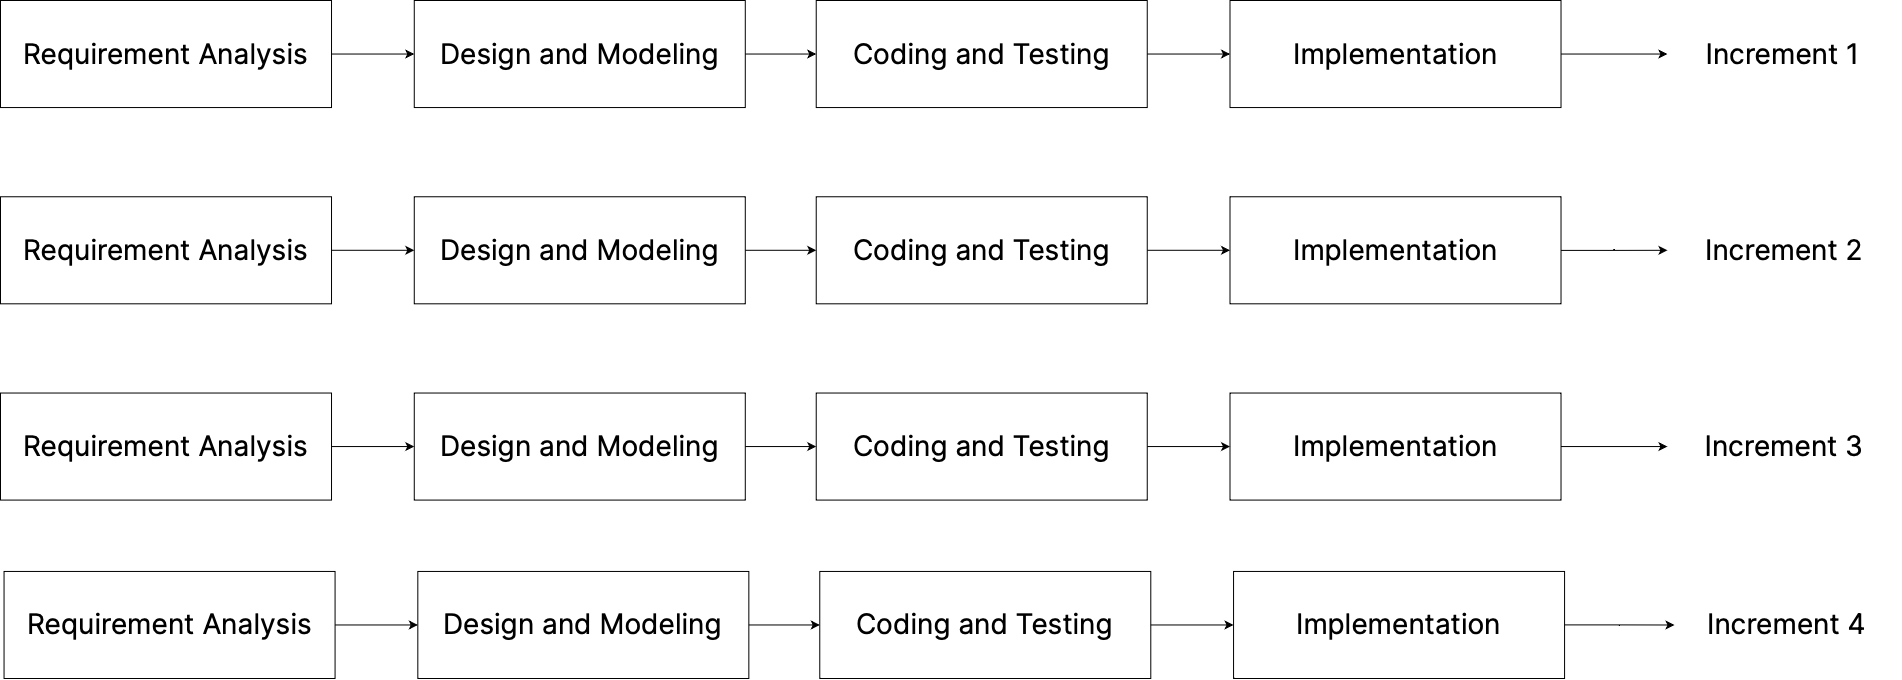
\includegraphics[width=6in, height=10in, keepaspectratio]{incremental.png}
			\label{incremental}
			\caption{Incremental Software model}
		\end{figure}
								
		
	
								
In the first increment, we initiated the project by focusing on two key areas. Firstly, we implemented a sentiment analysis model to process the Twitter data retrieved from the API. This model was designed to classify text as positive, negative, or neutral, providing valuable insights into the sentiment trends within the dataset. Additionally, we concurrently devoted substantial effort to the user interface (UI) design. This encompassed the creation of wireframes, mockups, and visual designs, ensuring an aesthetically pleasing and user-friendly experience. Moreover, we developed an engaging landing page that effectively showcased the product, providing potential users with essential information and compelling calls to action to explore further.


 Building upon the foundation laid in the first increment, we progressed to the second phase. Here, our primary focus was on enhancing the platform's security and user experience. We achieved this by integrating a seamless and secure user validation system through the integration of a robust API. This feature ensures that user data remains protected and accessible only to individuals who have their userID. Concurrently, we implemented an engagement metrics system to monitor and quantify user activity within the application. This system tracks metrics such as follower counts, following counts, favourite counts on the platform, providing valuable insights into user behavior and interaction patterns. Furthermore, we designed a user profile page, allowing users to conveniently manage their personal information and preferences.

 the third increment, we shifted our focus towards harnessing the power of social media data. This involved the systematic gathering of data pertaining to social media activity, with a particular emphasis on identifying popular hashtags within the industry. Additionally, we conducted a thorough analysis of top-performing tweets based on engagement metrics such as retweets, likes, and comments. This process allowed us to distill insights from successful content and optimize our approach accordingly. Lastly, we incorporated user feedback and usability testing outcomes to enhance the user interface, making iterative improvements that guarantee an intuitive and delightful user experience.


 In the fourth and final increment, we turned our attention to the presentation of analyzed data. We implemented advanced data visualization techniques to transform the processed Twitter data into insightful, interactive displays. These visualizations serve to convey trends, sentiment distributions, and other relevant information in a clear and engaging manner. Additionally, we focused on enhancing interactivity within the platform, enabling users to dynamically explore and interact with the visualized data. This increment represents the culmination of our efforts, delivering a robust, user-centric platform that empowers users to derive meaningful insights from Twitter data.




			      			      			      			      
		
								
		\clearpage
								
								
		\begin{flushleft}
			\fontsize{13}{15}\selectfont\textbf{3.2 System Architecture}
			\phantomsection
			\label{architecture}
		\end{flushleft}
								
		\begin{figure}[h]
			\centering
			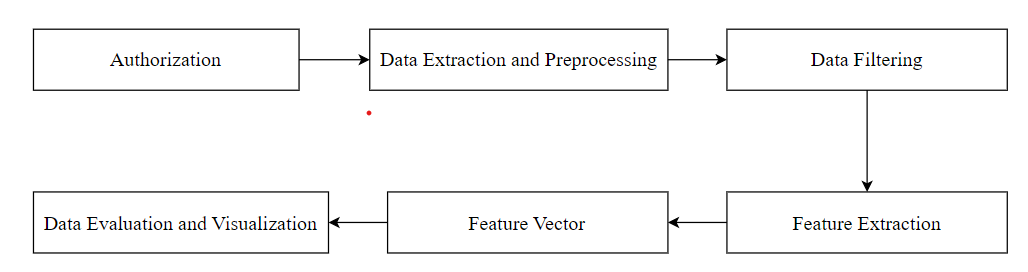
\includegraphics[width=6in, height=10in, keepaspectratio]{block_diagram.png}
			\label{block-diagram}
			\caption{Block Diagram of System Architecture}
		\end{figure}
								
								
		\begin{enumerate}
			\item \textbf{Authorization:} Set up authentication procedures to connect to the Twitter API safely and get the API keys and access tokens to authenticate app instance.
			      			      			      			           
			\item \textbf{Data Extraction and Prepossessing:} Use the Twitter API to retrieve pertinent information, such as user profiles, engagement metrics, and tweets efficiently get data, handle rate limitations and pagination given by the API. 
			      			      			      			           
			\item \textbf{Data Filtering:} For Data Filtering, We used available dataset on Huggingface which consist of two 
types of datasets(i.e Training Dataset and Testing Dataset). These datasets are 
balanced. And, Number of text in each dataset are 2084 and 2001 respectively. Our 
Datasets contains two categories that is Texts ,Labels. The Labels are of 3 types. Such 
as: Positive, Negative and Neutral. Originally, We used dataset from the link below. And, 
Used Pandas Library to perform filter operation so that the dataset meet the criteria for 
creation of our Sentiment Analysis model.Filters are applied to eliminate duplicate, irrelevant, and spam data to concentrate on pertinent tweets, and filter using particular criteria which may include language location or time frame.
			      			      			      			      
			\item \textbf{Feature Extraction:} From the tweet data, identifying and extracting the pertinent attributes such as text sentiment, user sentiment, hashtags, mentions, retweet count, and other features. Utilizing BERT for Nepali sentiment analysis, balanced datasets are loaded and preprocessed, with attribute extraction from tweet data.
			      			      			      			      
			      
			\item \textbf{Data Evaluation and Visualization: }Evaluate the sentiment (positive, negative, or neutral) of tweets, perform sentiment analysis on the text to present the findings of the investigation, employ data visualization techniques such as charts, graphs, and word clouds. Also acquire insights into trends, user sentiments, and engagement patterns, evaluate and interpret the data.
			      			      			      	     
		\end{enumerate}
								

    					
	
		\begin{flushleft}
			\fontsize{13}{15}\selectfont\textbf{3.3 Implemented Model}
			\phantomsection
			\label{bert}
		\end{flushleft}

   BERT (Bidirectional Encoder Representations from Transformers) is a Natural 
Language Processing Model proposed by researchers at Google Research in 2018. 
BERT model Architecture is based on  BERT-BASE and BERT-LARGE which are 
trained on a massive dataset. The BASE model is used to measure the performance of 
the architecture comparable to another architecture and the LARGE model produces 
state-of-the-art.

BERT is basically an Encoder stack of transformer architecture. A transformer 
architecture is an encoder-decoder network that uses self-attention on the encoder side 
and attention on the decoder side. BERTBASE has 12 layers in the Encoder stack while 
BERTLARGE has 24 layers in the Encoder stack. These are more than the Transformer 
architecture described in the original paper (6 encoder layers). 
BERT architectures 
(BASE and LARGE) also have larger feedforward networks (768 and 1024 hidden units 
respectively), and more attention heads (12 and 16 respectively) than the Transformer 
architecture suggested in the original paper. It contains 512 hidden units and 8 attention 
heads. BERTBASE contains 110M parameters while BERTLARGE has 340M 
parameters.

 This model takes the CLS token as input first, then it is followed by a sequence of words 
as input. Here CLS is a classification token. It then passes the input to the above layers. 
Each layer applies 
self-attention and passes the result through a feedforward network 
after then it hands off to the next encoder. The model outputs a vector of hidden size 
Untitled
 2
(768 for BERT BASE). If we want to output a classifier from this model we can take the 
output corresponding to the CLS token. Now, this trained vector can be used to perform a number of tasks such as 
classification, translation, etc.


  
		\newpage
		\begin{flushleft}
			\fontsize{13}{15}\selectfont\textbf{3.4 Use Case Diagram}
			\phantomsection
			\label{usecase}
		\end{flushleft}
								
		\begin{figure}[htbp]
			\centering
			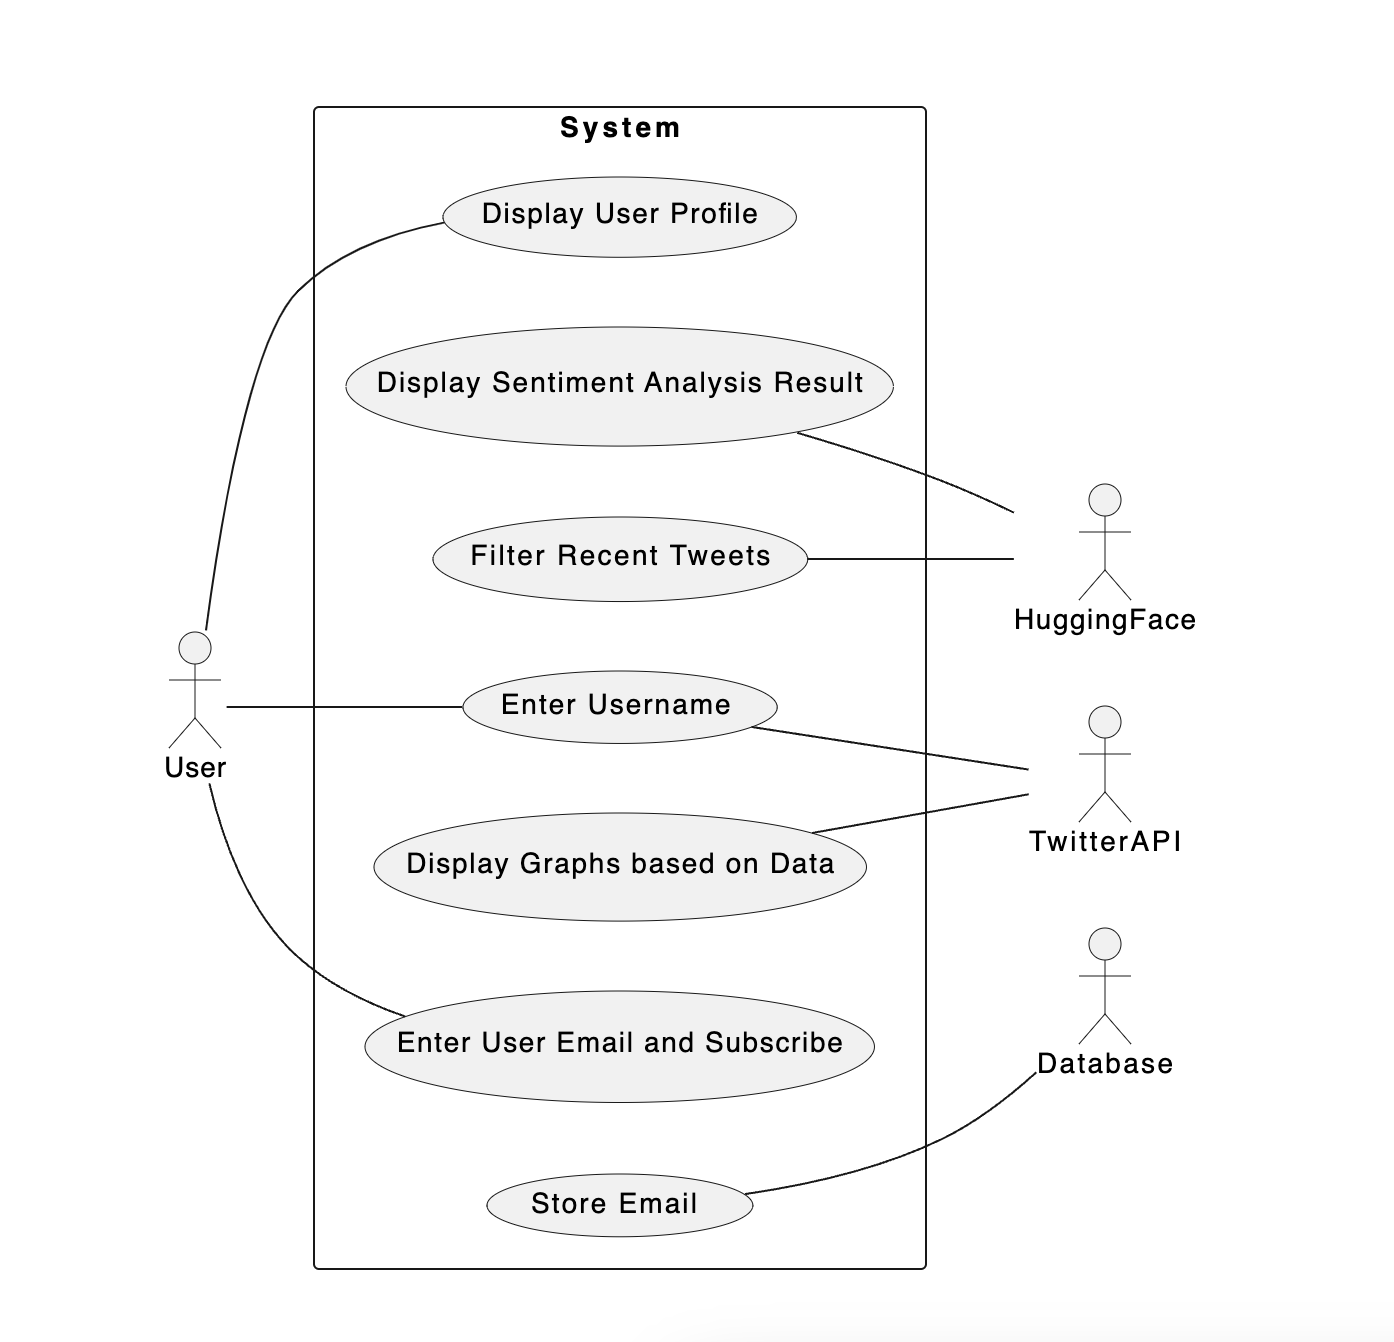
\includegraphics[width=6in, height=10in, keepaspectratio]{Usecase.png}
			\label{usecase_diagram}
			\caption{Use Case diagram}
		\end{figure}
								
				
	The use case diagram depicts the core functionalities of the project. The "User" interacts with the system through various use cases, including entering their username, filtering recent tweets, viewing sentiment analysis results, entering their email for subscription, and accessing their user profile. The system interfaces with external entities such as the "HuggingFace" API for sentiment analysis, "TwitterAPI" for data retrieval, and a "Database" for email storage. This diagram effectively illustrates the interactions and dependencies between the user and the system's key features.

\newpage
  
		\begin{flushleft}
			\fontsize{13}{15}\selectfont\textbf{3.5 Activity Diagram}
			\phantomsection
			\label{activity}
		\end{flushleft}
								
		\begin{figure}[htbp]
			\centering
			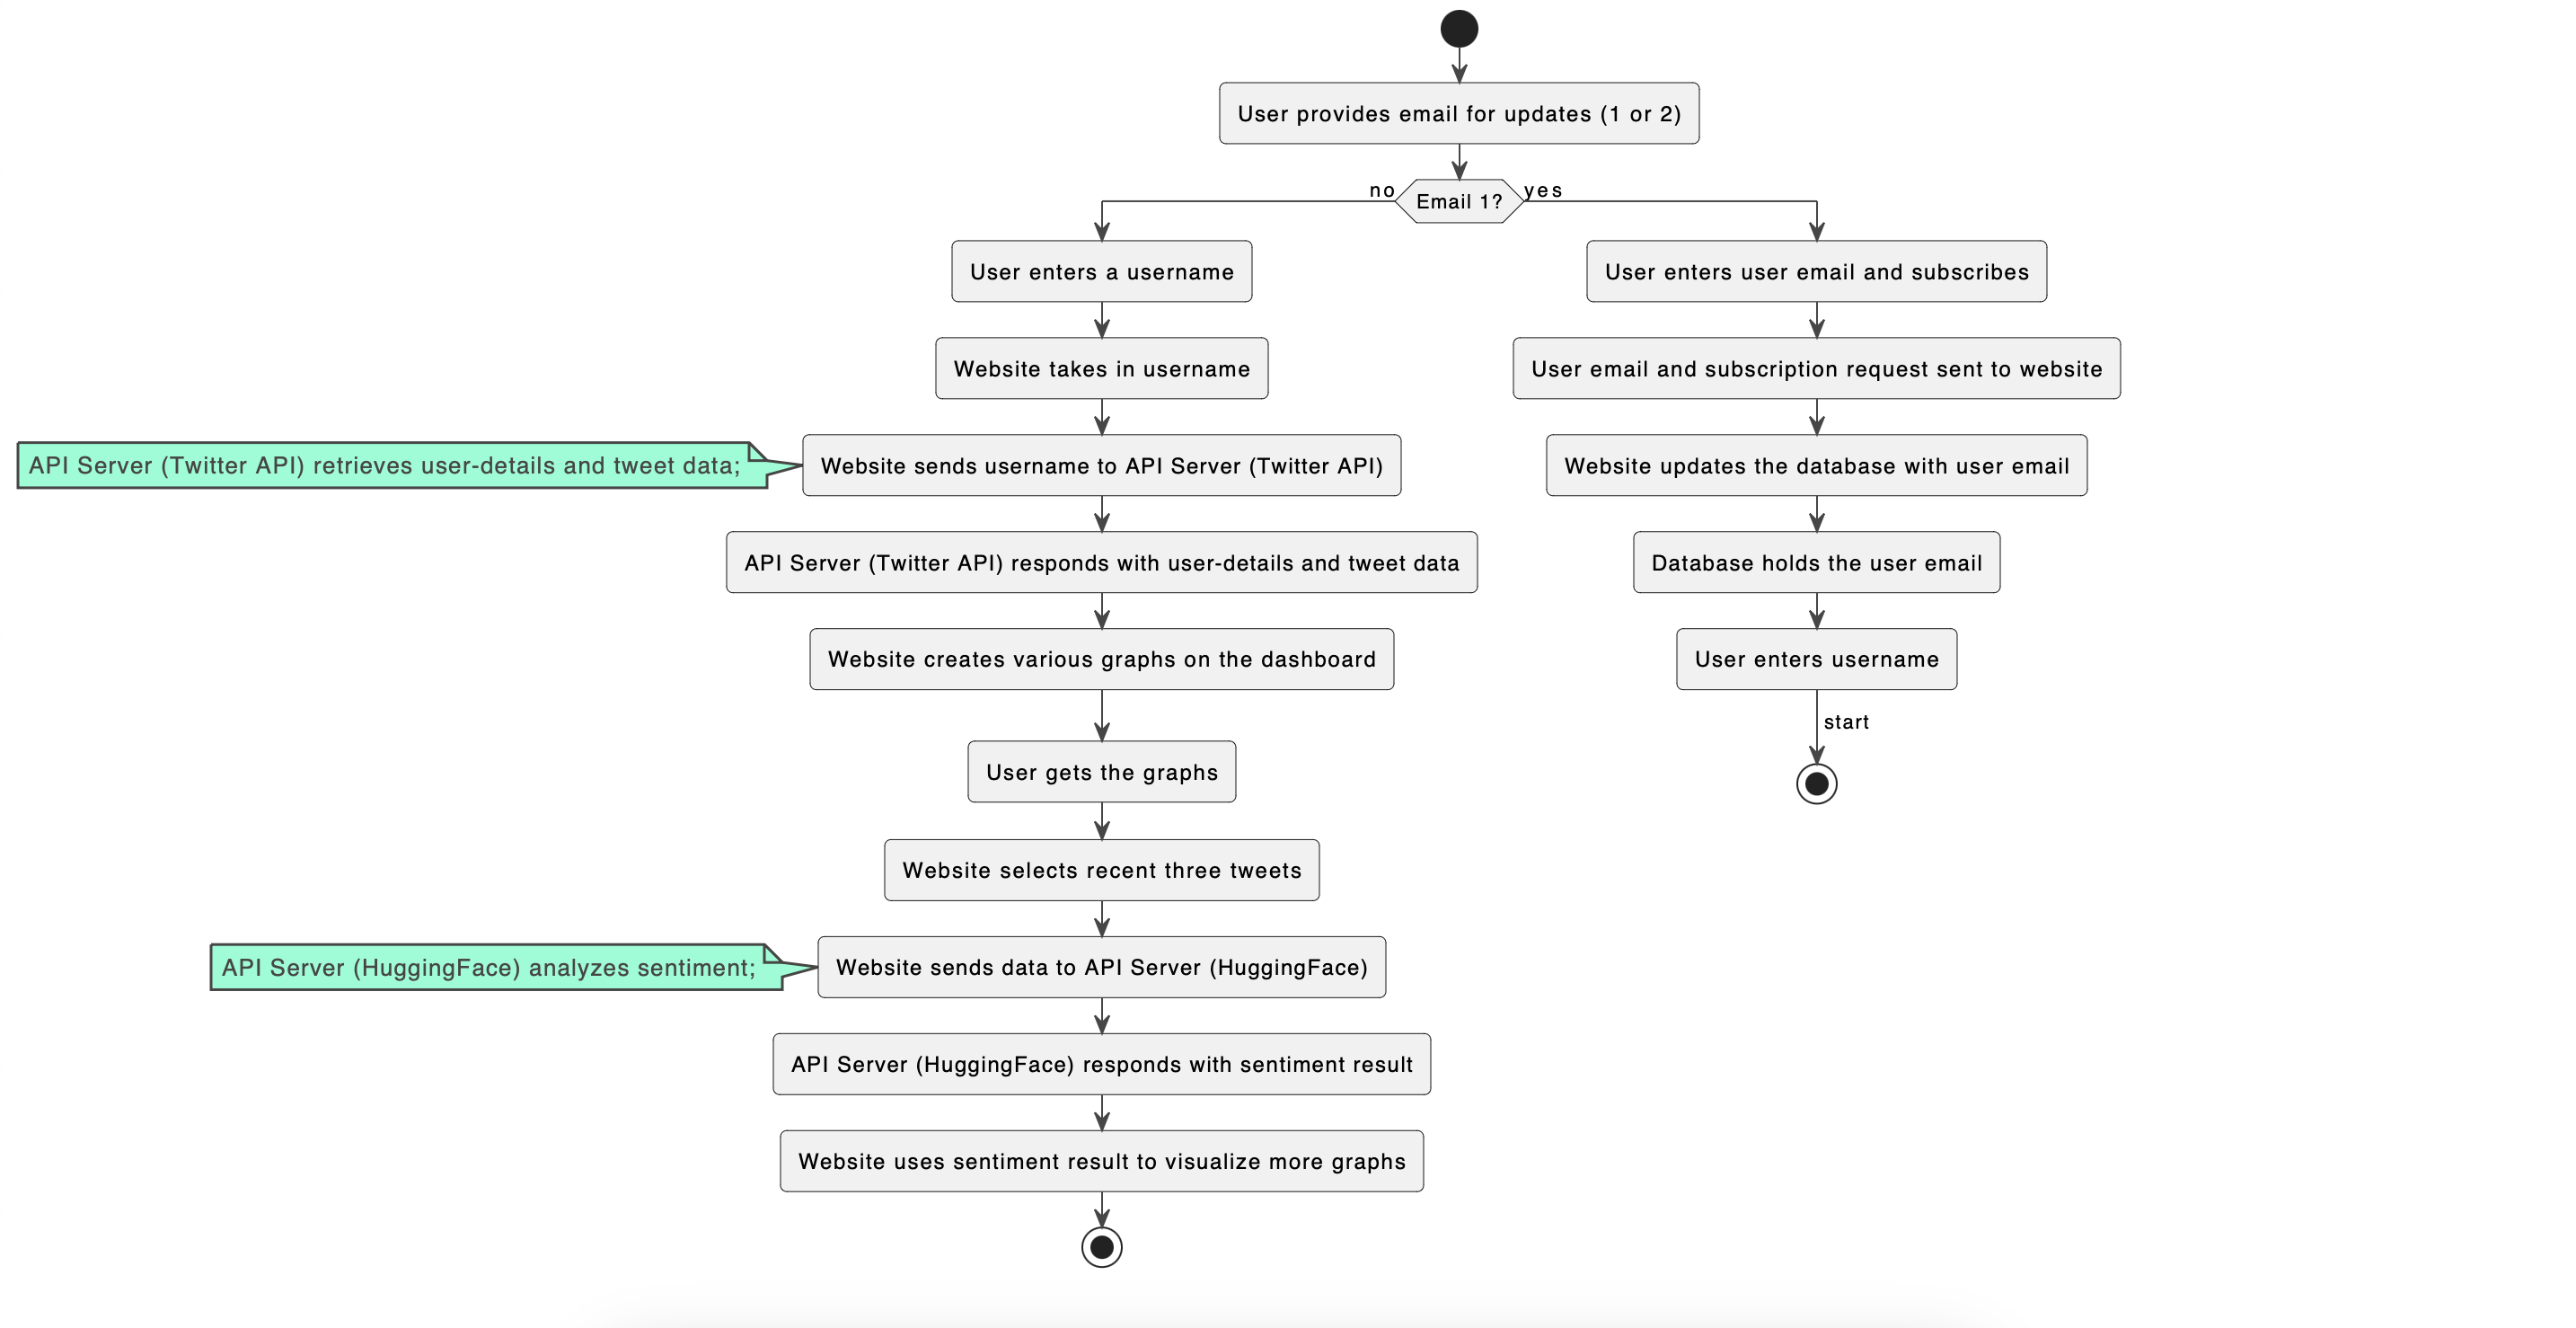
\includegraphics[width=7in, height=15in, keepaspectratio]{ActivityDiagram.png}
			\label{activitydiagram}
			\caption{Activity Diagram}
		\end{figure}

  The activity diagram outlines the flow of interactions in the project. Initially, the user decides whether to provide an email for updates or not. If not, they enter a username, which is sent to the Twitter API for data retrieval. Subsequently, the website generates graphs and displays them to the user. After selecting recent tweets, the HuggingFace API is employed for sentiment analysis. The sentiment result is then used to create additional visualizations. In the event of providing an email, the user's email is stored in the database, and they proceed to select a scenario, looping back to the start if desired.


  \newpage
		\begin{flushleft}
			\fontsize{13}{15}\selectfont\textbf{3.6 Sequence Diagram}
			\phantomsection
			\label{sequence}
		\end{flushleft}
								
		\begin{figure}[htbp]
			\centering
			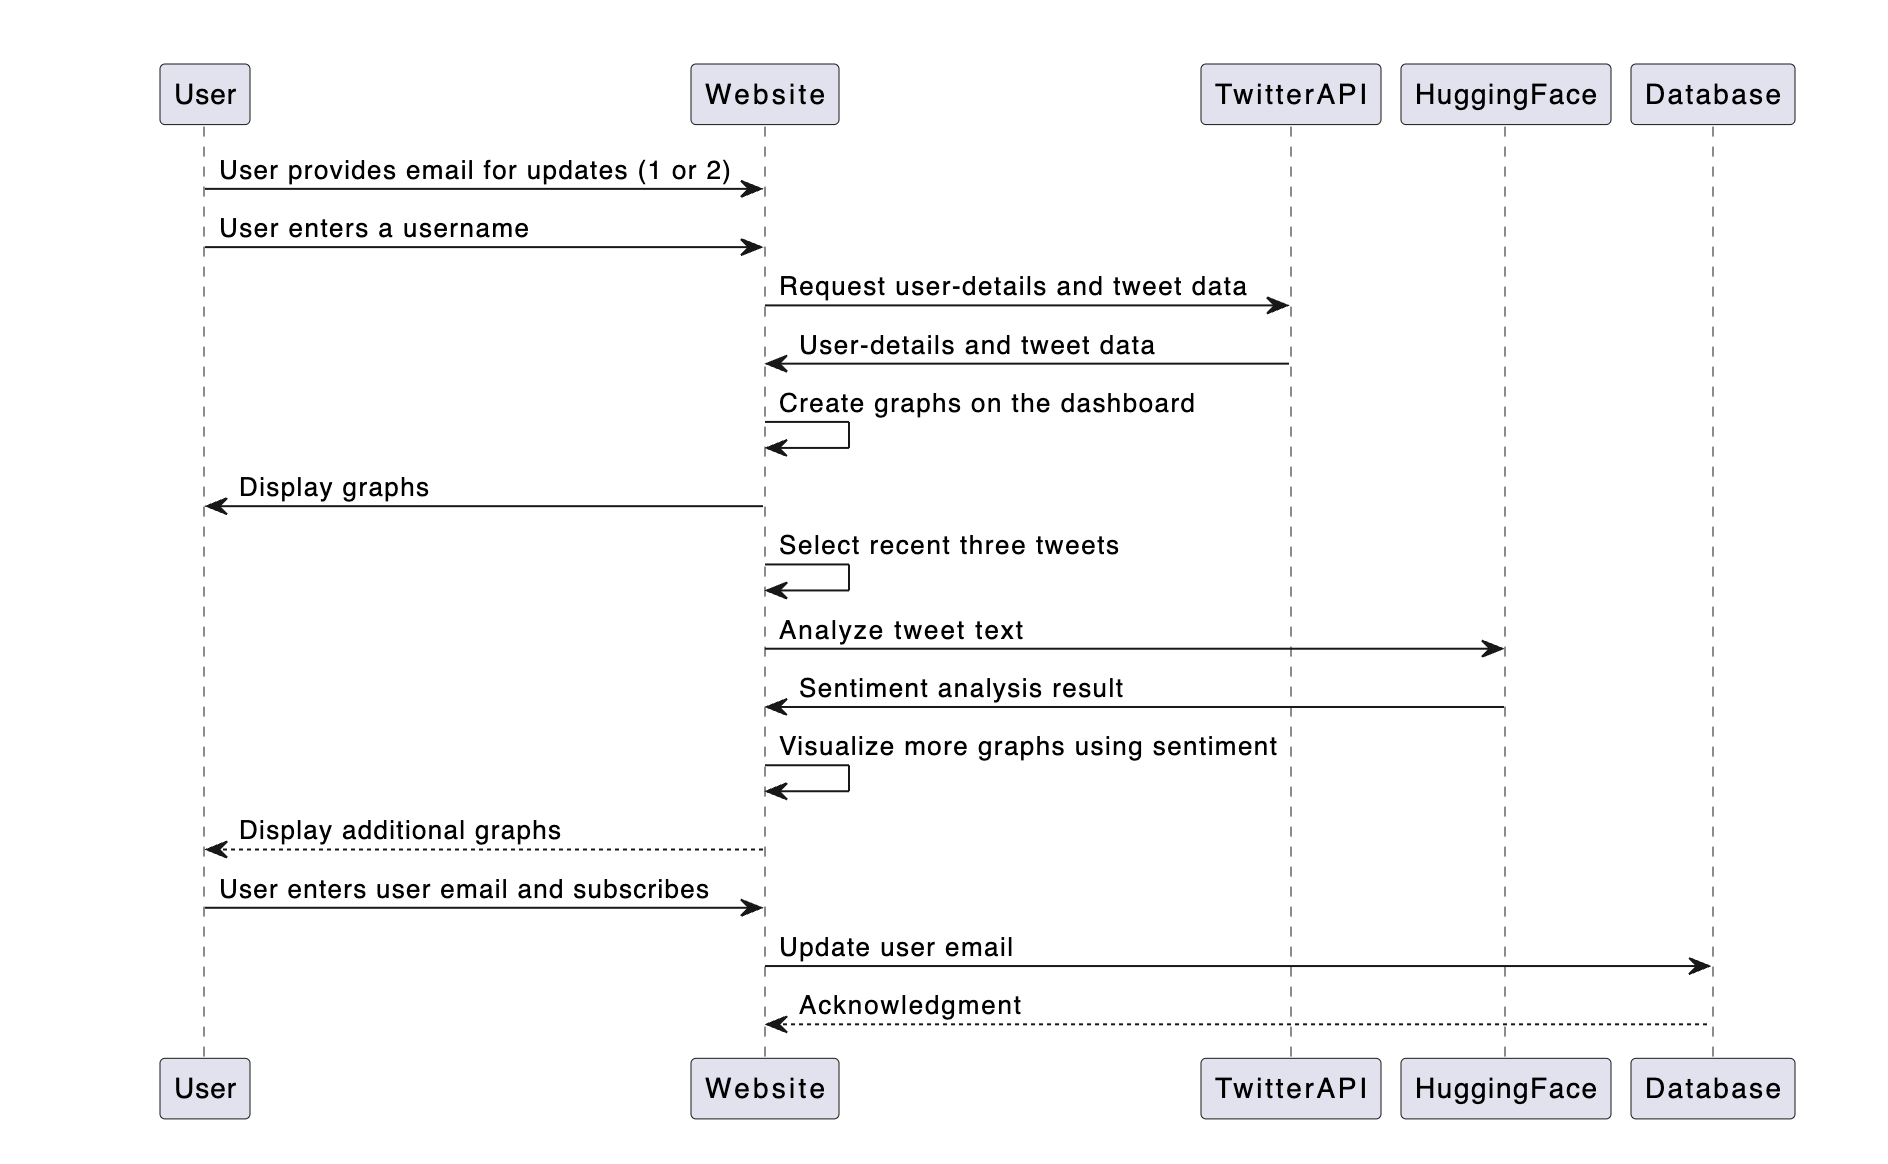
\includegraphics[width=6in, height=15in, keepaspectratio]{SequenceDiagram.png}
			\label{sequencediagram}
			\caption{Sequence Diagram}
		\end{figure}

  The sequence diagram illustrates the interactions within the project. Initially, the user provides an email for updates. They then enter a username, triggering the website to communicate with the Twitter API, retrieving user details and tweet data. The website subsequently creates graphs, displaying them to the user. Following this, recent tweets are selected and sent to the HuggingFace API for sentiment analysis. The sentiment result is utilized to generate additional visualizations. In an alternate scenario, the user can directly enter their email for subscription. This leads to the website updating the database with the user's email, concluding the interaction.
















  %                       4. REQUIREMENT ANALYSIS
								 
		\newpage
				
		\begin{flushleft}
			\fontsize{14}{16}\selectfont\textbf{4. REQUIREMENT ANALYSIS }
			\phantomsection
			\label{requirement}
		\end{flushleft}


    %                   4.1 FUNCTIONAL REQUIREMENTS

\begin{flushleft}
			\fontsize{13}{15}\selectfont\textbf{4.1 Functional Requirement}
			\phantomsection
			\label{fun}
		\end{flushleft}


 \begin{table}[h] 
\caption{Functional Requirements}
  \begin{center}
  \label{table}
\begin{tabular}{|c|p{5cm}|p{6cm}|}
\hline
\textbf{Serial Number} & \textbf{Functional Requirements} & \textbf{Description} \\
\hline
1 & API Integration & Utilize RAPID API for data retrieval, ensuring seamless access to Twitter information including tweets, followers, likes, and retweets. \\
\hline
2 & Data Visualization & Implement diverse visualization techniques (e.g., graphs, charts) for Twitter user data, prioritizing user-friendly representation. \\
\hline
3 & Sentiment Analysis & Incorporate hugging face Datasets in conjunction with a BERT model for effective sentiment analysis, distinguishing between positive, negative, and neutral reactions. \\
\hline
4 & Comprehensive Account Insights & Provide a comprehensive, well-organized display of a user's Twitter account statistics and metrics, encompassing details such as total tweets, followers, following, likes, and retweets. \\
\hline
5 & User Feedback Mechanism & Enable users to provide feedback based on their experience, fostering an avenue for continuous improvement and refinement of the platform. \\
\hline
\end{tabular}
\end{center}
\end{table}


%                        4.2  NON-FUNCTIONAL REQUIREMENTS
 \newpage
 
\begin{flushleft}
			\fontsize{13}{15}\selectfont\textbf{4.2 Non-Functional Requirement}
			\phantomsection
			\label{nonfun}
		\end{flushleft}

  \textbf{Performance:} The platform should be fast and responsive, capable of handling many users at once. Data retrieval and visualizations should happen quickly and smoothly.

\textbf{Usability:} The interface should be easy to use, making it simple for users to navigate and understand. User testing will be conducted to gather feedback and make improvements based on user experience.

\textbf{Reliability:} The platform should be available and dependable, with minimal downtime. Backup and recovery procedures will be in place to protect against data loss.

\textbf{Maintainability:} The source code will be kept straightforward for easy maintenance in case of any errors. The model and rendering functions will be separated, making it simple to track and correct changes.

\textbf{Portability and Compatibility:} The application will run smoothly on any operating system. It won't conflict with other resources or processes during operation.



%                                4.3 SOFTWARE REQUIREMENTS

\begin{flushleft}
			\fontsize{13}{15}\selectfont\textbf{4.3 Software Requirement}
			\phantomsection
			\label{soft}
		\end{flushleft}

\begin{flushleft}
			\fontsize{13}{15}\selectfont\textbf{4.3.1 Next.js}
			\phantomsection
			\label{next}
		\end{flushleft}
  Next.js is a powerful React framework that simplifies the creation of server-rendered web applications. It excels at optimizing performance with features like server-side rendering (SSR) and static site generation (SSG). Next.js seamlessly integrates with React, providing an efficient development environment for building dynamic and interactive web solutions.

  \begin{flushleft}
			\fontsize{13}{15}\selectfont\textbf{4.3.2 Redux}
			\phantomsection
			\label{redux}
		\end{flushleft}

 Redux is a state management library that works seamlessly with React and Next.js. It centralizes the application's state, making it easy to manage and modify data across various components. Redux promotes a predictable and manageable state flow, enhancing the maintainability and scalability of complex applications.

\newpage
 
\begin{flushleft}
			\fontsize{13}{15}\selectfont\textbf{4.3.3 Twitter API}
			\phantomsection
			\label{tweetapi}
		\end{flushleft}
 The Twitter API is a robust tool that allows developers to access and interact with Twitter's extensive dataset. With endpoints for user data, tweets, and interactions, it enables the integration of Twitter functionality into applications. Leveraging the Twitter API, developers can retrieve, post, and analyze tweets, enriching user experiences with real-time social media interaction.			


\begin{flushleft}
			\fontsize{13}{15}\selectfont\textbf{4.3.4 Torch}
			\phantomsection
			\label{torch}
		\end{flushleft}
 Torch is an open-source machine learning library widely used for numerical computations. It provides a dynamic computational graph system, making it particularly popular for deep learning tasks. Torch offers various tools and modules to efficiently build and train neural networks.

\begin{flushleft}
			\fontsize{13}{15}\selectfont\textbf{4.3.5 Pandas}
			\phantomsection
			\label{pandas}
		\end{flushleft}
 Pandas is a powerful Python library for data manipulation and analysis. It provides data structures like DataFrames, which allow for easy organization, filtering, and transformation of data. Pandas is commonly used for tasks such as data cleaning, exploration, and preparation in data science projects.


\begin{flushleft}
			\fontsize{13}{15}\selectfont\textbf{4.3.6 Transformers}
			\phantomsection
			\label{transform}
		\end{flushleft}
The Transformers library, developed by Hugging Face, is a comprehensive tool for natural language processing (NLP) tasks. It offers pre-trained models like BERT, GPT-2, and many others, which can be fine-tuned for specific NLP applications. Transformers has become a go-to library for advanced language understanding tasks.




\begin{flushleft}
			\fontsize{13}{15}\selectfont\textbf{4.3.7 Matplotlib}
			\phantomsection
			\label{mat}
		\end{flushleft}
 Matplotlib is a popular data visualization library in Python. It enables users to create a wide range of static, animated, and interactive plots and charts. Matplotlib is widely used in data analysis, scientific research, and engineering to visualize and communicate insights from datasets.

 \begin{flushleft}
			\fontsize{13}{15}\selectfont\textbf{4.3.8 LaTeX}
			\phantomsection
			\label{latex}
		\end{flushleft}
 LaTeX is widely used documentation preparation system for preparation of scientific documents, books and technical papers. It uses plain text for formatting unlike other document creation systems. The source code is compiled by a compeller to generate the printable/viewable document. The reason for using LaTeX for documentation was to learn this new form of documentation.

 \begin{flushleft}
			\fontsize{13}{15}\selectfont\textbf{4.3.9 MongoDB}
			\phantomsection
			\label{mongo}
		\end{flushleft}

MongoDB is a popular, open-source, NoSQL (non-relational) database system designed for storing and retrieving large volumes of unstructured or semi-structured data. It uses a flexible document-oriented data model, which means data is stored in flexible, JSON-like BSON (Binary JSON) format. MongoDB is known for its scalability, high performance, and ease of horizontal scaling across multiple servers. It is widely used in modern web applications, mobile apps, and other scenarios where flexible, high-volume data storage and retrieval is crucial.

		












  
%                        IMPLEMENTATION DETAILS
		\newpage
		
								
		\begin{flushleft}
			\fontsize{14}{16}\selectfont\textbf{5. IMPLEMENTAION DETAILS}
			\phantomsection
			\label{implementation}
		\end{flushleft}






  \begin{flushleft}
			\fontsize{13}{15}\selectfont\textbf{5.1 AI Model}
			\phantomsection
			\label{ai}
		\end{flushleft}


  \begin{flushleft}
			\fontsize{13}{15}\selectfont\textbf{5.1.1 DataSet}
			\phantomsection
			\label{data}
		\end{flushleft}
  The dataset used for training and testing the sentiment analysis model is a balanced dataset in CSV format. The dataset is loaded using the pandas library. The training dataset consists of 2084 balanced data, and the test dataset consists of 2001 balanced data. Label 0 = Negative, Label 1 = Positive, Label 2 = Neutral \cite{shushant_nepali_sentiment}


  \begin{figure}[htbp]
			\centering
			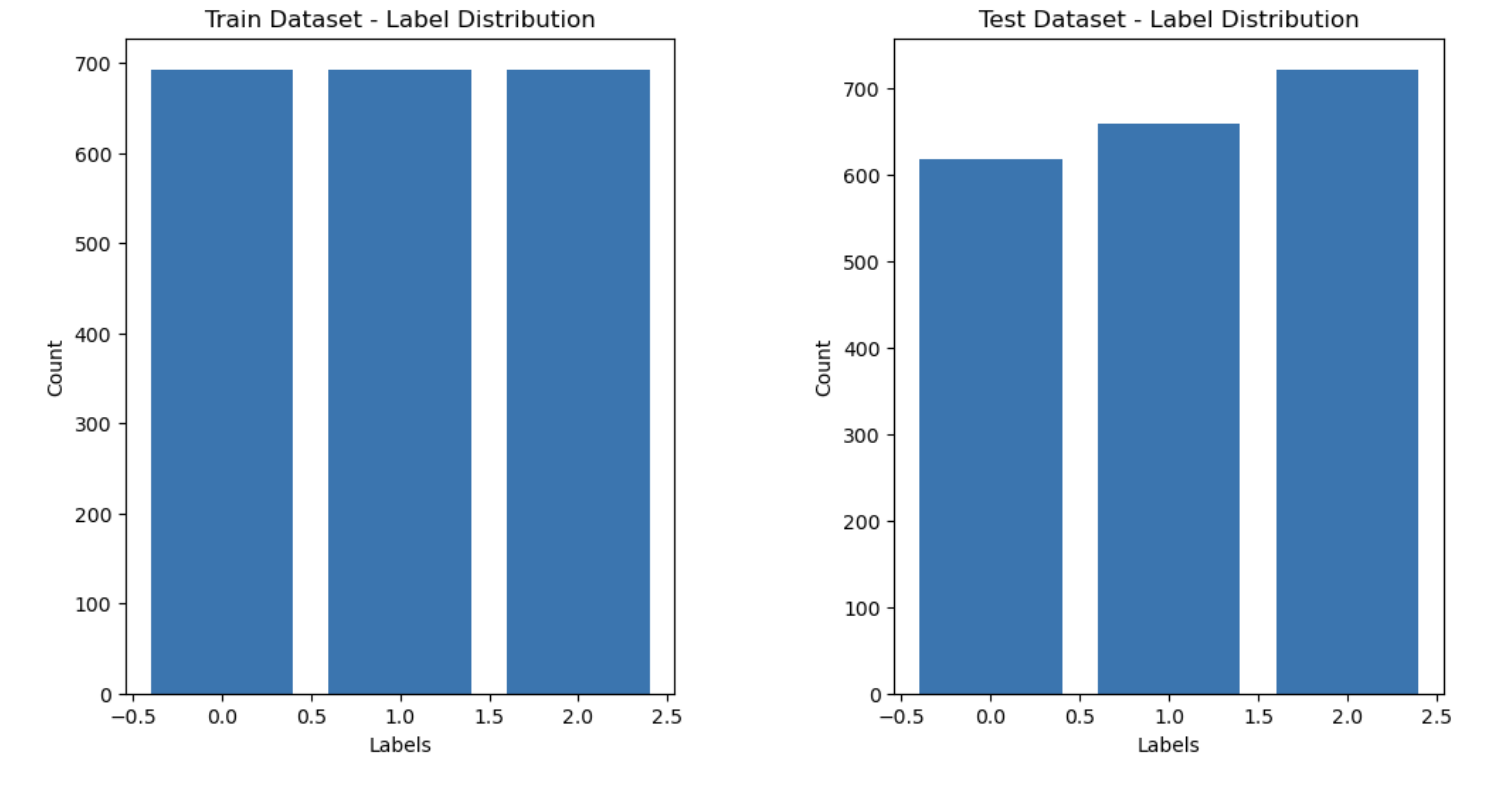
\includegraphics[width=6in, height=15in, keepaspectratio]{dataset.png}
			\label{dataset}
			\caption{Dataset }
		\end{figure}
  


  \begin{flushleft}
			\fontsize{13}{15}\selectfont\textbf{5.1.2 Model}
			\phantomsection
			\label{model}
		\end{flushleft}
The BERT model is used for sequence classification and is loaded from the bert-base-multilingual-uncased pre-trained model. The model is initialized with \texttt{num\_labels} = 3 since we have three sentiment classes: positive, negative, and neutral.

  
\newpage

    \begin{flushleft}
			\fontsize{13}{15}\selectfont\textbf{5.1.3 Preprocessing}
			\phantomsection
			\label{preprocess}
		\end{flushleft}
				
The dataset is preprocessed using the NepaliSentimentDataset class. The class takes the texts, labels, tokenizer, and maximum sequence length as inputs. The texts are preprocessed using regular expressions to remove special characters, usernames, and extra whitespace. The tokenizer from the Hugging Face transformers library is used to tokenize the texts and convert them into input IDs and attention masks. The preprocessed data is returned as a dictionary with the input IDs, attention masks, and labels.



\begin{flushleft}
			\fontsize{13}{15}\selectfont\textbf{5.1.4 Training}
			\phantomsection
			\label{train}
		\end{flushleft}


The model is trained using the train-model function. The function takes the model, train dataloader, and test dataloader as inputs. The model is trained for 10 epochs with an early stopping mechanism. The AdamW optimizer is used with a learning rate of 2e-5 and epsilon value of 1e-8. The function also includes additional connection layers before the classification layer of the BERT model. After each epoch, the model is evaluated on the test dataset.



  \begin{flushleft}
			\fontsize{13}{15}\selectfont\textbf{5.2 User Interface Development}
			\phantomsection
			\label{user}
		\end{flushleft}

In the development of our frontend, we opted for NextJS as our framework of choice, leveraging TypeScript for enhanced code quality and maintainability. NextJS provided a sturdy foundation, allowing us to build a modern web application with efficiency and precision. Complementing this, Tailwind CSS played a pivotal role in our styling approach. This utility-first framework not only facilitated a cohesive and visually appealing user interface but also ensured responsiveness across various devices and screen sizes, enhancing the overall user experience.

Form management was seamlessly handled through React Hooks/Form, enabling us to create interactive and dynamic forms. This approach proved instrumental in gathering User Experiences and business queries, contributing to a user-centric design philosophy. API data management was a critical component, and we relied on Tanstack for this task. Its capabilities in handling data fetching from external sources ensured a performant application, delivering data with precision and speed.

For state management, Redux became our cornerstone. Its implementation provided a robust cache storage system, guaranteeing consistent and accessible data throughout the application. This significantly contributed to a smooth and uninterrupted user experience, particularly in dynamic components and interactions. Additionally, Recharts played a vital role in visualizing data within our dashboard. This visual element added a layer of interactivity and engagement to the application.

The integration of Twitter API through Rapid API was a standout feature of our frontend implementation. This integration allowed us to seamlessly retrieve user details, providing a personalized touch through the Profile Page. Users experienced a tailored interface, thereby enhancing engagement and overall satisfaction. Structurally, our web application encompasses two core sections. The Landing Page serves as the initial point of contact, introducing users to the application's purpose and functionality. On the other hand, the Dashboard Pages house the central functionality.Dashboard contains profile page and preferences page within it. The Profile Page displays user details retrieved from the Twitter API, enriching the user experience with personalized content. The Preferences Page, meanwhile, hosts the feedback form, facilitating user experience providing a channel for valuable insights.

  


  \begin{flushleft}
			\fontsize{13}{15}\selectfont\textbf{5.3 Database}
			\phantomsection
			\label{database}
		\end{flushleft}
  In this project, we leveraged MongoDB Atlas as our chosen database solution. A cluster was established within a newly created project, and crucial credentials, including the cluster's ID, password, and database name ('subscriptions'), were securely stored as environment variables. To enforce email validation, we integrated a regular expression-based validation system into the contact model, adhering to the defined schema. This model was designed for the purpose of storing contact information, encompassing attributes such as email addresses and date entries. Using Mongoose, we implemented a 'connectDB' function to manage the database connection. This function verifies the existence of a connection and, if successful, establishes it using the provided 'mongoDB-URI' from the environment variables. Upon successful connection, a confirmation message, 'db-Connected', is logged. This robust database setup ensures reliable data management throughout the project.















 
				    











   
		  
%                        RESULT AND ANALYSIS
		\newpage
				
		\begin{flushleft}
			\fontsize{14}{16}\selectfont\textbf{6. RESULT AND ANALYSIS}
			\phantomsection
			\label{result}
		\end{flushleft}

  
  \begin{flushleft}
			\fontsize{13}{15}\selectfont\textbf{6.1 Training Progress and Evaluation Metrics}
			\phantomsection
			\label{train}
		\end{flushleft}



This section provides insights into the training progress of the sentiment analysis model and includes graphs showing the loss values and accuracy values throughout the training process.


\begin{flushleft}
			\fontsize{13}{15}\selectfont\textbf{6.1.1 Loss Value Graph}
			\phantomsection
			\label{lvg}
		\end{flushleft}

The graph below displays the training progress by showing the variation in the loss values across different epochs. It helps visualize the convergence of the model during training.

\begin{figure}[htbp]
			\centering
			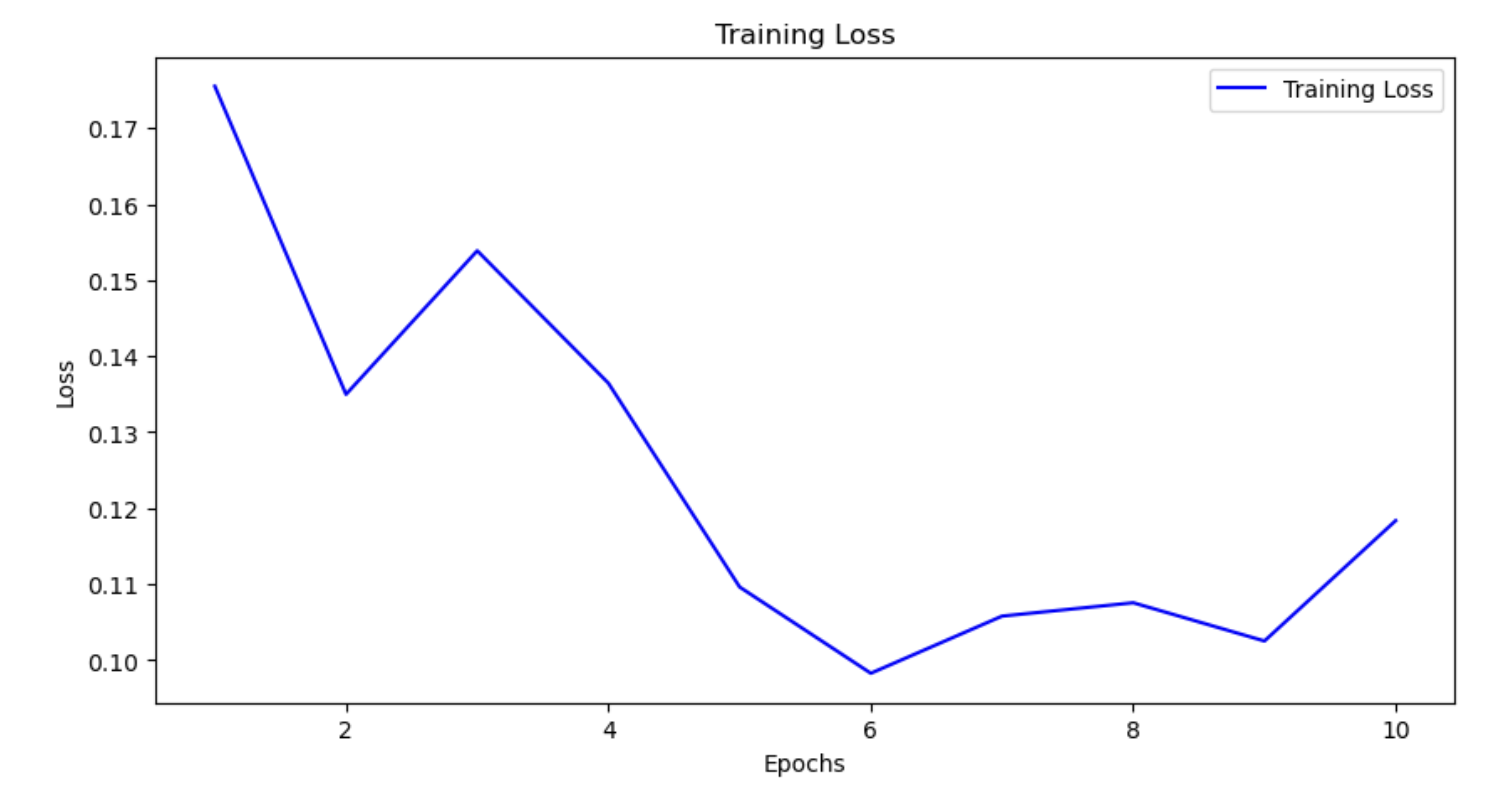
\includegraphics[width=6in, height=15in, keepaspectratio]{trainingloss.png}
			\label{loss}
			\caption{Loss Value Graph }
		\end{figure}
  


\newpage
  \begin{flushleft}
			\fontsize{13}{15}\selectfont\textbf{6.1.2 Accuracy Value Graph}
			\phantomsection
			\label{avg}
		\end{flushleft}

  These graphs provide a visual representation of the training progress and performance of the sentiment analysis model, allowing for better understanding and analysis of the results.

\begin{figure}[htbp]
			\centering
			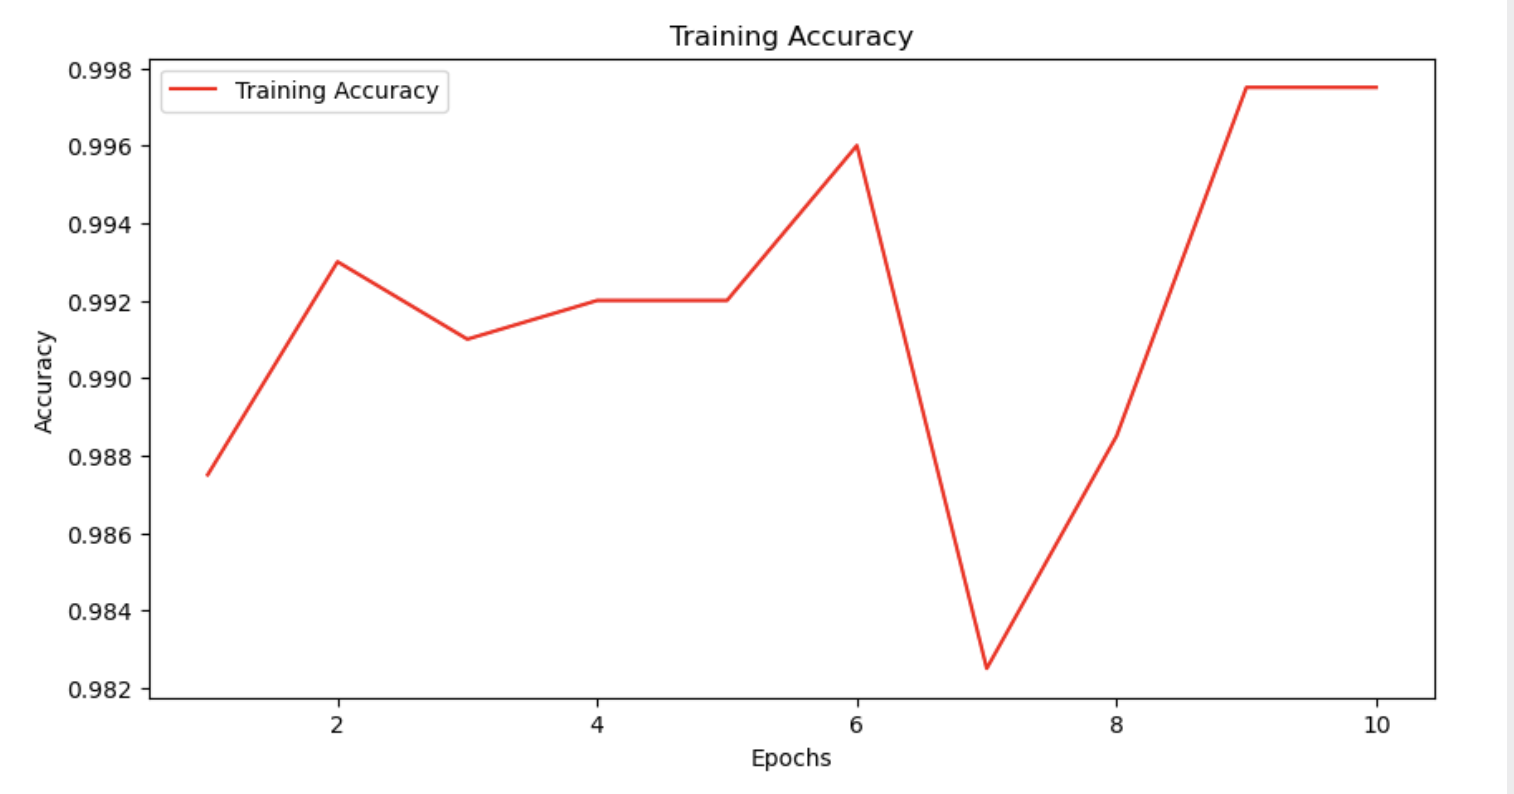
\includegraphics[width=6in, height=15in, keepaspectratio]{trainingacc.png}
			\label{acc}
			\caption{Accuracy Value Graph }
		\end{figure}

After training, the trained model achieves an accuracy of 99.75\% on the test dataset.


\begin{flushleft}
			\fontsize{13}{15}\selectfont\textbf{6.2 Data Visualisation}
			\phantomsection
			\label{dv}
		\end{flushleft}

The project encompasses a dynamic dashboard tailored for visualizing Twitter data through a series of insightful graphs and charts. This component serves as a central hub for aggregating and presenting key metrics extracted from real-time Twitter feeds. The underlying architecture leverages the Twitter API to seamlessly retrieve live data, ensuring the dashboard remains updated with the latest trends and sentiments. To facilitate the creation of the graphical representations, the richarts library has been integrated, offering a diverse set of tools and features for crafting visually appealing visualizations. These range from bar charts and line graphs to pie charts, allowing for a comprehensive representation of the data's dimensions. The implementation process begins by initializing the Twitter API with the requisite authentication credentials, establishing a secure connection for data retrieval. Subsequently, the fetched Twitter data is meticulously processed and passed onto richarts, where it undergoes transformation into visually meaningful representations. The resulting visualizations are seamlessly integrated into the dashboard, providing users with a clear and intuitive overview of the trends and sentiments emanating from the Twitter sphere. This synthesis of real-time data retrieval, robust visualization capabilities, and user-friendly presentation culminates in a powerful tool for comprehensive Twitter data analysis. The project report emphasizes this integration of technologies and methodologies, underscoring the pivotal role played by the richarts library in enhancing the project's visual output and analytical capabilities.





 \begin{figure}[htbp]
			\centering
			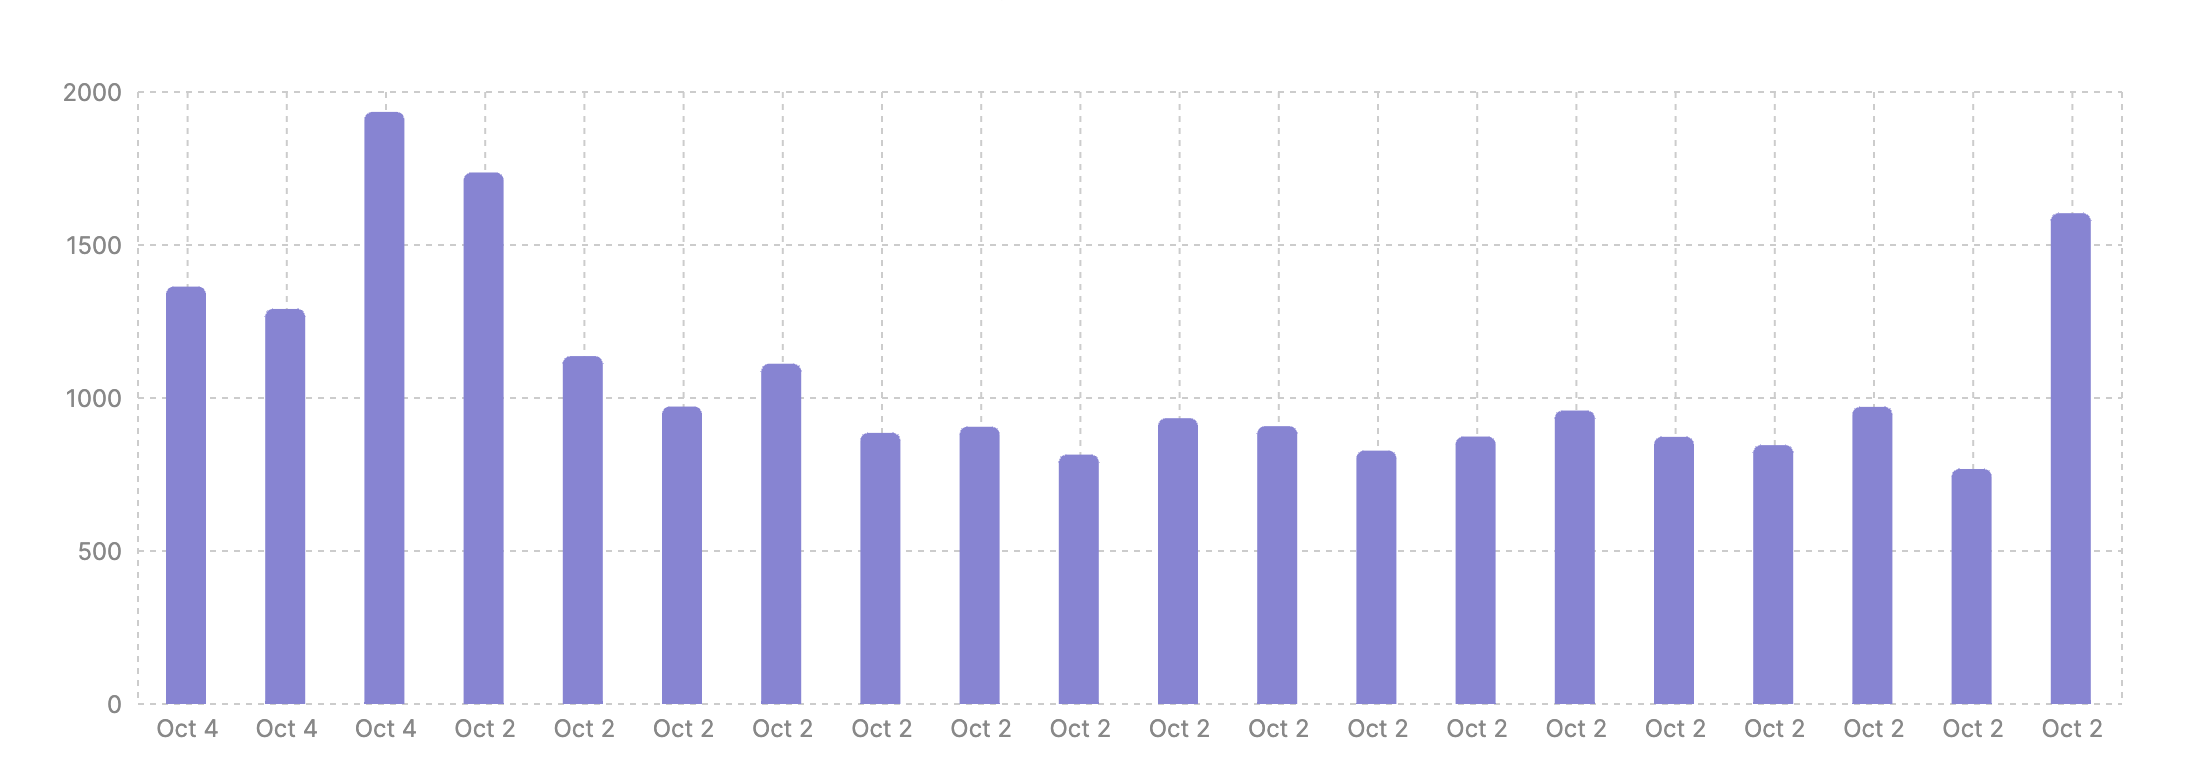
\includegraphics[width=6in, height=15in, keepaspectratio]{tweet_performance.png}
			\label{per}
			\caption{Tweet performance graph}
		\end{figure}
  




  
 \begin{figure}[htbp]
			\centering
			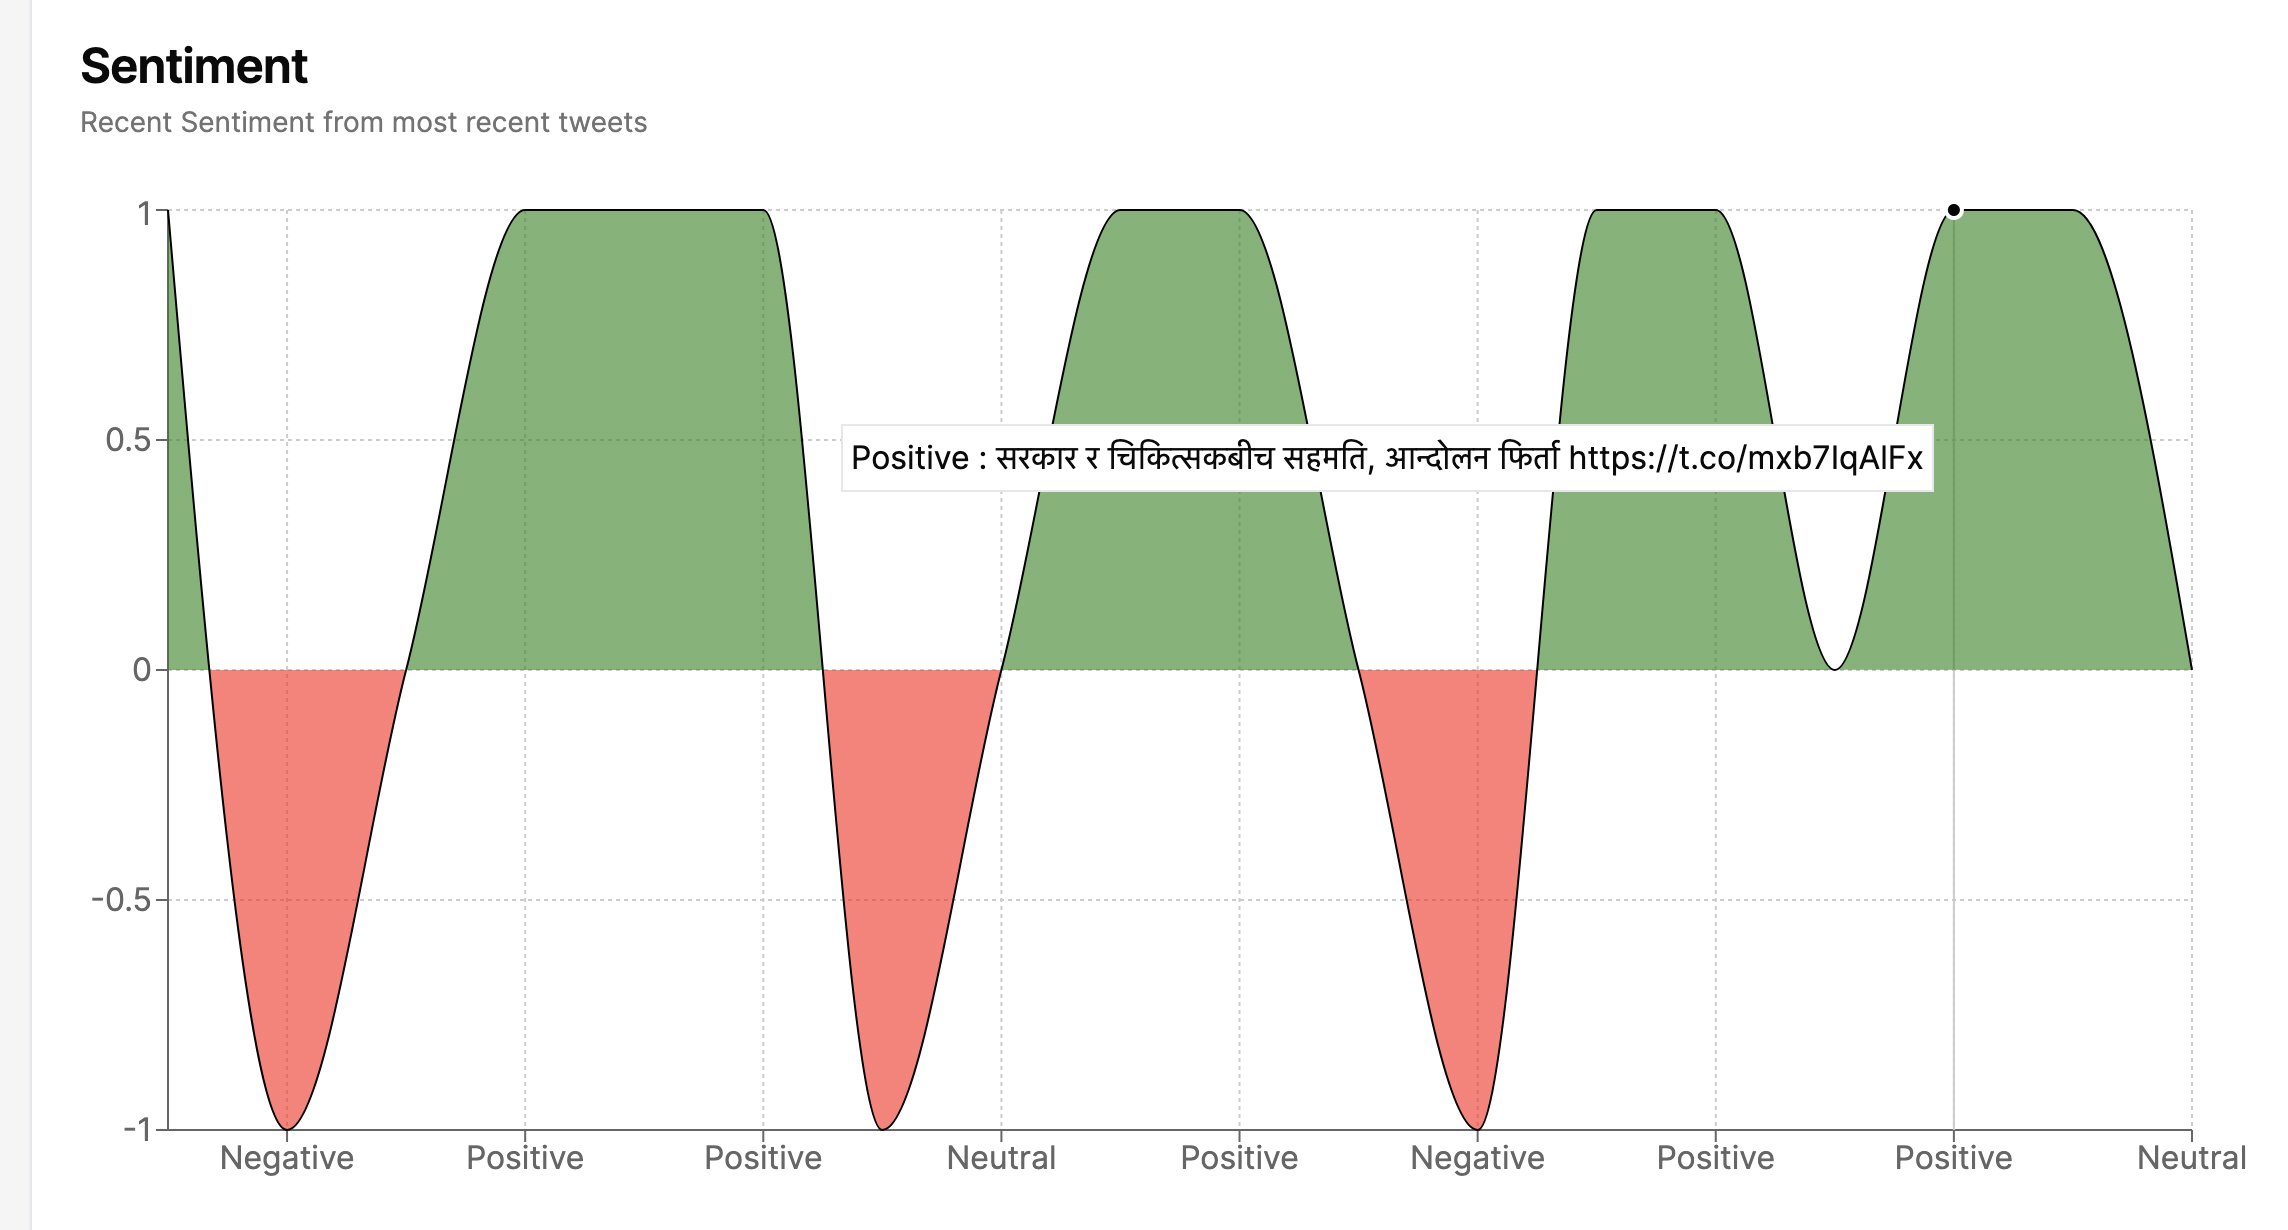
\includegraphics[width=6in, height=15in, keepaspectratio]{sentiment.png}
			\label{sent}
			\caption{Sentiment Analysis Graph}
		\end{figure}
  \clearpage


















 %                              CONCLUSIONS
		\newpage
				
		\begin{flushleft}
			\fontsize{14}{16}\selectfont\textbf{7. CONCLUSIONS}
			\phantomsection
			\label{conclusion}
		\end{flushleft}
				
	In conclusion, I-NEPAL represents a significant advancement in the field of social media analytics, especially in terms of being sensitive to the particular requirements of the Nepali environment. It provides users with in-depth insights into their Twitter accounts by utilizing the Twitter API, presenting data in a simple, user-friendly way, and providing sophisticated sentiment analysis for tweets written in Nepali. Users have access to a powerful tool through I-NEPAL to improve their Twitter strategy, resulting in deeper interactions with their audience. This platform not only contributes to the development of digital communication and analysis in the area, it also fills a critical gap in Nepal's social media landscape. I-NEPAL is positioned to become an essential tool for everyone wishing to optimize their potential thanks to its user-friendly interface and comprehensive functionality.
				
		
		            








   
   


%                           FUTURE ENHANCEMENTS

		\newpage
				
		\begin{flushleft}
			\fontsize{14}{16}\selectfont\textbf{8. FUTURE ENHANCEMENTS}
			\phantomsection
			\label{future}
		\end{flushleft}

The limitations of the current API are our main priority as we pursue future improvements. We hope to access a variety of cutting-edge features and real-time insights by purchasing the premium version of Twitter's official API. This will revolutionize how consumers interact with their social media data. Users will be able to monitor and engage with their audience in a more dynamic and effective way thanks to this improvement, which offers a seamless experience.

We also have a commitment to improving platform support and enhancing customisation. Real-time engagement data must be implemented, and customized user options must be offered. We plan to expand I-Nepal's functionality beyond Twitter to include well-known social media sites like Instagram and Facebook, giving users a complete picture of their online presence. Last but not least, we are actively creating a dedicated application for both Android and iOS in recognition of the changing mobile-centric landscape. By doing this, consumers will be able to access their insights while on the go, offering a unified and simple user experience across all devices. These developments demonstrate our commitment to offering a state-of-the-art social media analytics solution specifically designed to meet the requirements of the Nepali context.

				

	












    
					
%                        PROJECT TASK AND TIME SCHEDULE
		\newpage
								
		\begin{flushleft}
			\fontsize{14}{16}\selectfont\textbf{9. PROJECT TASK AND TIME SCHEDULE}
			\phantomsection
			\label{task}
		\end{flushleft}
								
		\begin{figure}[htbp]
			\centering
			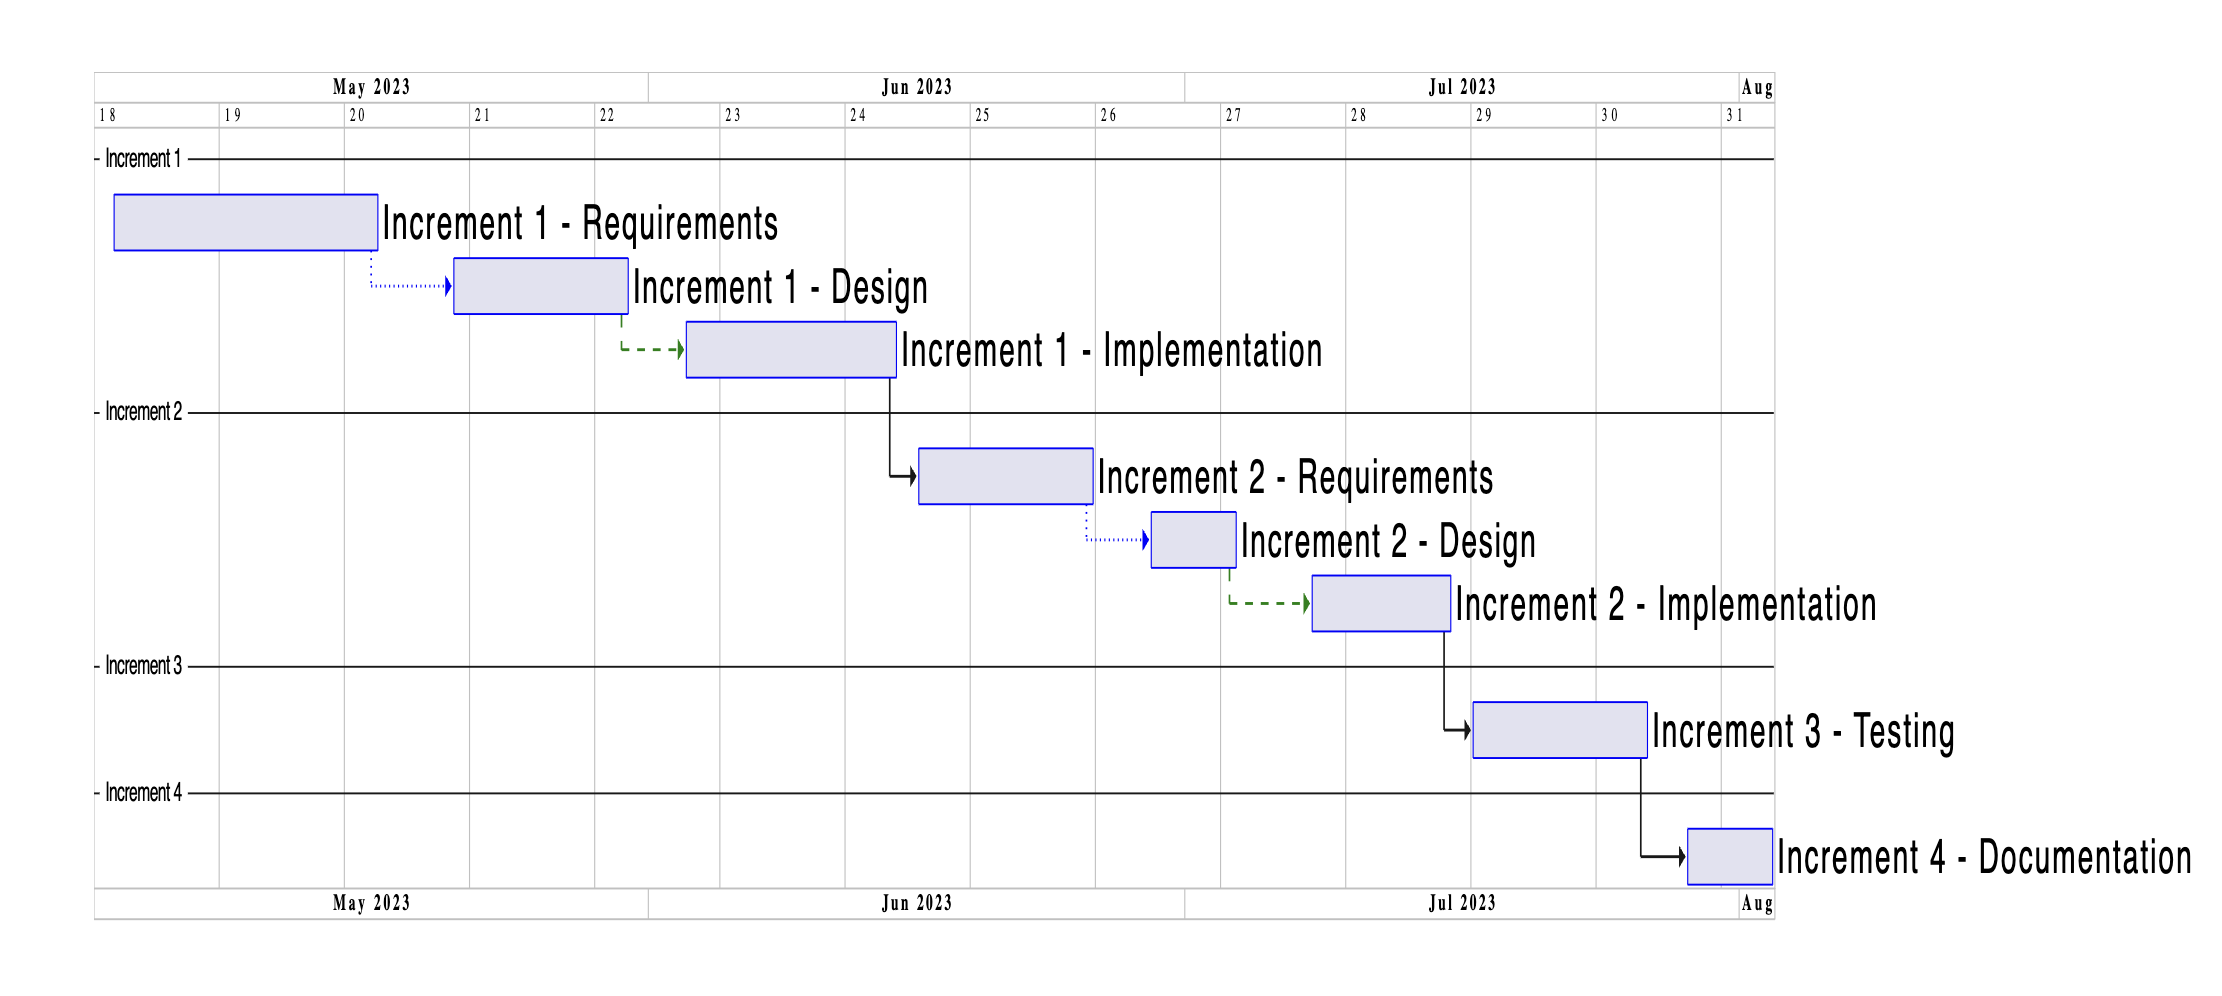
\includegraphics[width=\textwidth,height=\textheight,keepaspectratio]{Gantt-chart.png}
			\caption{Gantt chart}
			\label{gantt}
		\end{figure}
				
















    
%              REFERENCES
		\newpage
	

\label{reference}
 
\bibliographystyle{unsrt}
\bibliography{references}





\end{document}